% 컴파일 방법: cd docs && /Library/TeX/texbin/latexmk -xelatex research_blog_stellar_classification.tex
\documentclass[11pt,a4paper]{article}

% ---------------------------------------------------------------------------
% 한글 및 폰트 설정 (XeLaTeX + kotex)
% ---------------------------------------------------------------------------
\usepackage{kotex}
\setmainhangulfont{AppleMyungjo}[
  BoldFont={Apple SD Gothic Neo Bold},
  AutoFakeSlant=0.16
]
\setsanshangulfont{Apple SD Gothic Neo}[
  BoldFont={Apple SD Gothic Neo Bold},
  AutoFakeSlant=0.16
]
\setmonohangulfont{Apple SD Gothic Neo}

% ---------------------------------------------------------------------------
% 레이아웃 및 패키지
% ---------------------------------------------------------------------------
\usepackage[top=25mm,bottom=25mm,left=22mm,right=22mm,headheight=23pt]{geometry}
\usepackage{graphicx}
\usepackage{booktabs}
\usepackage{tabularx}
\usepackage{array}
\usepackage{amsmath,amssymb}
\usepackage{xcolor}
\usepackage{tcolorbox}
\tcbuselibrary{skins,breakable}
\usepackage{tikz}
\usetikzlibrary{arrows.meta,positioning,shapes.geometric,calc,fit,backgrounds}
\usepackage{caption}
\usepackage{subcaption}
\usepackage{fancyhdr}
\usepackage{enumitem}
\usepackage{float}
\usepackage[colorlinks=true,linkcolor=NavyAccent,urlcolor=BlueAccent,citecolor=NavyAccent]{hyperref}

\graphicspath{{../DL/figures/}{../EDL/figures/}}

% ---------------------------------------------------------------------------
% 컬러 팔레트 (Research Blog 스타일)
% ---------------------------------------------------------------------------
\definecolor{NavyAccent}{HTML}{0F2C59}
\definecolor{BlueAccent}{HTML}{0969DA}
\definecolor{TealAccent}{HTML}{1A7F37}
\definecolor{RedAccent}{HTML}{CF222E}
\definecolor{AmberAccent}{HTML}{9A6700}
\definecolor{SoftBg}{HTML}{F6F8FA}
\definecolor{SoftBlueBg}{HTML}{EEF5FF}
\definecolor{SoftGreenBg}{HTML}{EEFAF2}
\definecolor{SoftAmberBg}{HTML}{FFF8E6}
\definecolor{BorderGray}{HTML}{D0D7DE}
\definecolor{MutedText}{HTML}{57606A}

% ---------------------------------------------------------------------------
% 문단, 캡션, 헤더/푸터 스타일
% ---------------------------------------------------------------------------
\setlength{\parindent}{0pt}
\setlength{\parskip}{6pt}
\renewcommand{\baselinestretch}{1.32}

\captionsetup{
  font={small},
  labelfont={bf,color=NavyAccent},
  margin=6mm
}

\pagestyle{fancy}
\fancyhf{}
\fancyhead[L]{\small\sffamily\textcolor{MutedText}{Research Blog \,|\, Stellar Classification: Deep Learning vs.\ Evolutionary Neural Networks}}
\fancyhead[R]{\small\sffamily\textcolor{MutedText}{\thepage}}
\renewcommand{\headrulewidth}{0.4pt}
\renewcommand{\headrule}{\hbox to\headwidth{\color{BorderGray}\leaders\hrule height \headrulewidth\hfill}}

% ---------------------------------------------------------------------------
% 커스텀 콜아웃 박스 정의
% ---------------------------------------------------------------------------
\newtcolorbox{insightbox}[1]{
  enhanced,
  breakable,
  colback=SoftBlueBg,
  colframe=BlueAccent,
  boxrule=0.7pt,
  leftrule=3.5pt,
  arc=3pt,
  top=7pt, bottom=7pt, left=10pt, right=10pt,
  fonttitle=\sffamily\bfseries\small,
  coltitle=NavyAccent,
  attach title to upper={\par\smallskip},
  title={#1}
}

\newtcolorbox{discoverybox}[1]{
  enhanced,
  breakable,
  colback=SoftGreenBg,
  colframe=TealAccent,
  boxrule=0.7pt,
  leftrule=3.5pt,
  arc=3pt,
  top=7pt, bottom=7pt, left=10pt, right=10pt,
  fonttitle=\sffamily\bfseries\small,
  coltitle=TealAccent!85!black,
  attach title to upper={\par\smallskip},
  title={#1}
}

\newtcolorbox{cautionbox}[1]{
  enhanced,
  breakable,
  colback=SoftAmberBg,
  colframe=AmberAccent,
  boxrule=0.7pt,
  leftrule=3.5pt,
  arc=3pt,
  top=7pt, bottom=7pt, left=10pt, right=10pt,
  fonttitle=\sffamily\bfseries\small,
  coltitle=AmberAccent!90!black,
  attach title to upper={\par\smallskip},
  title={#1}
}

\newtcolorbox{codebox}[1]{
  enhanced,
  breakable,
  colback=SoftBg,
  colframe=BorderGray,
  boxrule=0.6pt,
  arc=3pt,
  top=6pt, bottom=6pt, left=10pt, right=10pt,
  fonttitle=\sffamily\bfseries\footnotesize,
  coltitle=MutedText,
  colbacktitle=BorderGray!40,
  title={#1}
}

% ---------------------------------------------------------------------------
% 문서 시작
% ---------------------------------------------------------------------------
\begin{document}

% 타이틀 배너 영역
\begin{tcolorbox}[
  enhanced,
  colback=NavyAccent,
  colframe=NavyAccent,
  arc=4pt,
  top=14pt, bottom=14pt, left=14pt, right=14pt
]
  {\sffamily\footnotesize\bfseries\textcolor{SoftBlueBg!85!white}{RESEARCH BLOG \& TECHNICAL STORYTELLING \;\textbullet\; ASTROINFORMATICS \& NEUROEVOLUTION}}\\[6pt]
  {\sffamily\LARGE\bfseries\textcolor{white}{밤하늘의 10만 개 빛을 분류하는 두 가지 인공지능 이야기}}\\[4pt]
  {\sffamily\large\textcolor{SoftBlueBg}{정통 딥러닝(DL)부터 스스로 뇌 구조를 진화시키는 신경망(EDL/TWEANN)까지}}\\[10pt]
  {\sffamily\small\textcolor{BorderGray}{저자: 이인수 \quad|\quad 데이터셋: SDSS-17 (100,000 천체 관측 기록) \quad|\quad 작성일: 2026년 11월}}
\end{tcolorbox}

\vspace{4pt}

\begin{insightbox}{프롤로그 요약 --- 이 글에서 다루는 핵심 이야기}
\emph{``멀리서 반짝이는 저 작은 빛은 우리 은하 안의 \textbf{별(Star)}일까, 수억 개의 별이 모인 외부 \textbf{은하(Galaxy)}일까, 아니면 초기 우주의 초대질량 블랙홀이 뿜어내는 \textbf{퀘이사(Quasar)}일까?''}

본 리서치 블로그는 슬론 디지털 전천 탐사(\textbf{SDSS-17})가 관측한 \textbf{100,000개의 천체 데이터}를 바탕으로, 천체를 $97.4\% \sim 97.9\%$의 높은 정확도로 분류해 내는 두 가지 상반된 인공지능 패러다임의 연구 여정을 일반 독자의 눈높이에서 소개합니다.
\begin{enumerate}[leftmargin=18pt, itemsep=2pt, topsep=3pt]
  \item \textbf{정통 딥러닝과 이종 앙상블 (\texttt{DL/})}: 천문학적 도메인 지식(색지수와 적색편이)을 바탕으로 정교하게 다듬은 역전파 다층 신경망(\textbf{97.37\%})과 그래디언트 부스팅 트리 결합(\textbf{97.88\%})의 여정
  \item \textbf{스스로 뇌 구조와 가중치를 진화시키는 진화 신경망 (\texttt{EDL/})}: 미분 공식 대신 생물학적 진화 원리(돌연변이$\cdot$교배$\cdot$적자생존)를 통해 \textbf{인간이 설계하지 않은 3층 스킵 연결 신경망 구조를 스스로 발명}하며 기존 딥러닝 단일 모델을 뛰어넘기(\textbf{97.45\%})까지의 탐구 기록
\end{enumerate}

\vspace{3pt}
\noindent\textbf{안내 (제3의 패러다임 GravNet 연계)}: 본 블로그는 프로젝트의 1단계 연구 성과인 \textbf{역전파 딥러닝(\texttt{DL/}) vs. 위상·가중치 진화 신경망(\texttt{EDL/})}의 2대 패러다임 비교를 다룹니다. 이후 제1원리 천체역학 기반으로 새롭게 개발된 제3의 무역전파 모델 \textbf{시공간 중력장 궤도 신경망(\texttt{GravNet/})}에 대한 학술 논문 및 상세 보고서는 \href{run:gravnet_ieee.pdf}{\texttt{gravnet\_ieee.pdf}} 및 \href{run:gravnet_research_report.pdf}{\texttt{gravnet\_research\_report.pdf}}를 참조하십시오.
\end{insightbox}

\tableofcontents
\vspace{6pt}
\noindent\textcolor{BorderGray}{\rule{\textwidth}{0.6pt}}

% ===========================================================================
\section{프롤로그: 밤하늘의 점 10만 개를 구분하는 법}
% ===========================================================================

망원경으로 밤하늘을 촬영하면 수없이 많은 빛의 점들이 찍힙니다. 맨눈이나 단순한 흑백 사진만으로는 그 빛이 우리 은하 내부의 가까운 \textbf{별(STAR)}인지, 아득한 우주 너머 수천억 개의 별이 모인 \textbf{은하(GALAXY)}인지, 혹은 초기 우주의 중심 블랙홀이 은하 전체보다 밝게 빛나는 \textbf{퀘이사(QSO, Quasar)}인지 구별하기 어렵습니다.

우리가 분석한 \textbf{SDSS-17 (Sloan Digital Sky Survey Data Release 17)} 데이터셋에는 총 \textbf{100,000개}의 실제 천체 관측 기록이 담겨 있습니다.

\begin{table}[H]
\centering
\caption{SDSS-17 데이터셋의 세 가지 천체 클래스 구성과 천문학적 특징}
\label{tab:classes}
\small
\begin{tabularx}{\textwidth}{lrrX}
\toprule
\textbf{천체 종류 (Class)} & \textbf{데이터 수} & \textbf{비중} & \textbf{천체물리학적 정체 및 관측 특징} \\
\midrule
\textbf{은하 (GALAXY)} & 59,445개 & \textbf{59.4\%} & 수억$\sim$수조 개의 항성과 성운이 중력으로 묶인 거대 천체 집단 \\
\textbf{별 (STAR)} & 21,594개 & \textbf{21.6\%} & 우리 은하 내부에서 핵융합으로 스스로 빛을 내는 항성 (지구와 매우 가까움) \\
\textbf{퀘이사 (QSO)} & 18,961개 & \textbf{19.0\%} & 초기 우주의 초대질량 블랙홀 주변 강착원반에서 뿜어져 나오는 극도로 밝은 활동성 은하핵 \\
\bottomrule
\end{tabularx}
\end{table}

천문학자들은 이 천체들의 정체를 밝히기 위해 크게 두 가지 물리량을 측정합니다.

\begin{itemize}[leftmargin=16pt, itemsep=3pt]
  \item \textbf{5가지 색상 필터를 통과한 밝기 (측광 등급, $u, g, r, i, z$)}: 자외선($u$), 초록빛($g$), 붉은빛($r$), 근적외선($i, z$) 5개 파장 대역에서 천체의 겉보기 등급을 측정합니다. (등급 숫자가 작을수록 밝고, 숫자가 클수록 어두운 천체입니다.)
  \item \textbf{분광 적색편이 (Redshift, $z_{\text{spec}}$)}: 우주는 팽창하고 있기 때문에 지구에서 멀리 떨어진 천체일수록 그 천체가 방출한 빛의 파장이 길어지며 붉은색 쪽으로 치우칩니다. 즉, \textbf{적색편이(\texttt{redshift})는 천체가 지구로부터 얼마나 먼 우주에 있는지를 알려주는 `우주 거리계'}입니다.
\end{itemize}

% ===========================================================================
\section{데이터 탐험: ``이상치(Outlier)인 줄 알았는데 보물이었다!''}
% ===========================================================================

데이터 과학의 첫걸음은 결측치와 이상치(Outlier)를 점검하는 일입니다. 10만 개 행을 전수 검사한 결과, 딱 한 행(79,543번째 관측치)에 센서 결측 센티널 값(\texttt{-9999})이 기록되어 있어 이를 제거하고 \textbf{99,999개}의 깨끗한 천체 데이터를 확보했습니다.

그런데 표준 통계 기법($1.5 \times \text{IQR}$ 사분위수 범위 규칙)으로 이상치를 탐지하자 놀라운 현상이 발견되었습니다. \textbf{\texttt{redshift}(적색편이) 변수에서 무려 8,990개(전체의 9.0\%)가 `통계적 이상치'로 지목된 것}입니다.

\begin{cautionbox}{초보 데이터 분석가가 빠지기 쉬운 함정}
교과서적인 전처리 규칙만 기계적으로 적용해 \emph{``박스플롯 바깥에 찍힌 8,990개의 이상치를 노이즈로 보고 삭제하자!''}라고 결정했다면 어떻게 되었을까요? 아래 교차 분석 결과가 그 해답을 보여줍니다.
\end{cautionbox}

우리는 이상치를 지우는 대신, 이상치로 분류된 8,990개의 천체가 실제로 어떤 클래스에 속하는지 역추적했습니다.

\begin{figure}[H]
  \centering
  \begin{subfigure}[t]{0.48\textwidth}
    \centering
    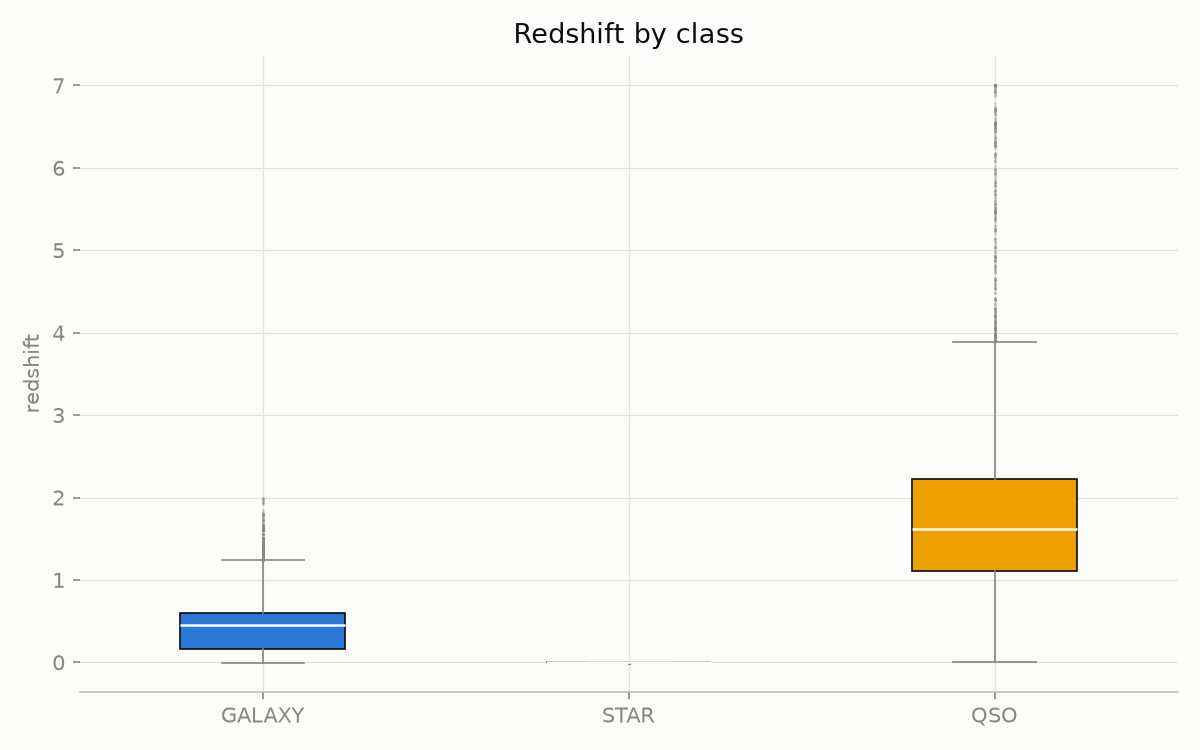
\includegraphics[width=\textwidth]{redshift_by_class.png}
    \caption{클래스별 적색편이(\texttt{redshift}) 분포}
    \label{fig:redshift}
  \end{subfigure}\hfill
  \begin{subfigure}[t]{0.48\textwidth}
    \centering
    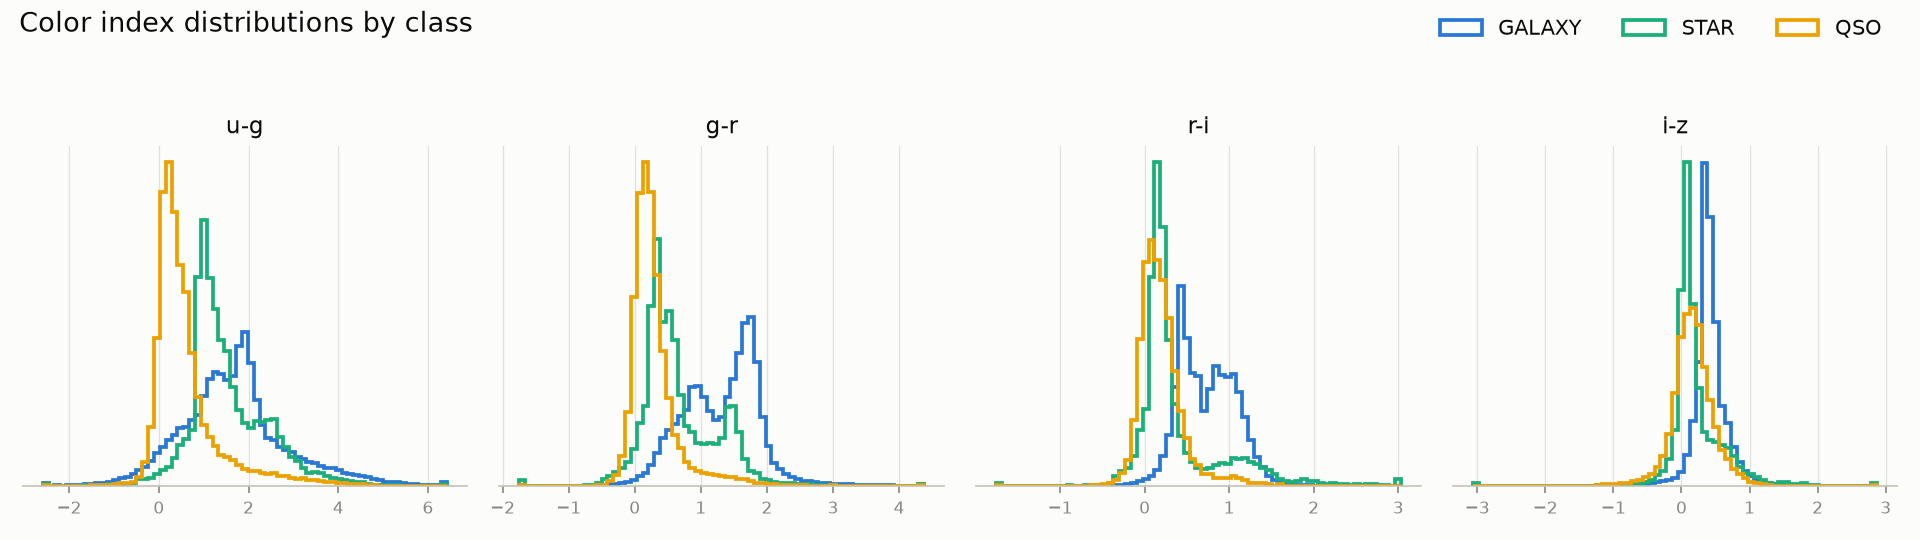
\includegraphics[width=\textwidth]{color_indices_by_class.png}
    \caption{파생 색지수($u-g, g-r, r-i, i-z$) 밀도 분포}
    \label{fig:colors}
  \end{subfigure}
  \caption{천체물리학적 도메인 지식이 드러나는 핵심 분포. 적색편이의 긴 꼬리는 퀘이사(QSO)의 고유 신호이며, 인접 필터 간 밝기 차이인 색지수(Color Index)는 세 천체의 온도 차이를 선명하게 분리합니다.}
\end{figure}

결과는 극적이었습니다(그림~\ref{fig:redshift}):
\begin{itemize}[leftmargin=16pt, itemsep=2pt]
  \item \texttt{redshift} 이상치로 지목된 \textbf{8,990개 중 무려 99.6\%(8,956개)가 퀘이사(QSO)}였습니다!
  \item 우리 은하 내부의 \textbf{별(STAR)}은 거리가 매우 가까워 $\text{redshift} \approx 0$에 모여 있고, 일반 \textbf{은하(GALAXY)}는 중앙값 $0.42$ 부근에 분포하는 반면, 초기 우주 끝에 자리한 \textbf{퀘이사(QSO)}는 적색편이가 $1.6$에서 최대 $7.01$까지 길게 뻗어 있었던 것입니다.
  \item 즉, 통계적으로는 `극단값'처럼 보였지만 실제로는 \textbf{``이 천체는 거의 확실히 퀘이사다!''라고 알려주는 결정적 보물 신호}였습니다. 우리는 이를 보존하되, 긴 우측 꼬리를 신경망이 안정적으로 학습하도록 $\log(1 + \text{redshift})$ 변환을 적용했습니다.
\end{itemize}

\subsection{천체의 `표면 온도'를 읽어내는 마법의 파생 변수: 색지수 (Color Index)}

여기에 천문학 도메인 지식을 하나 더 접목했습니다. 인접한 두 필터의 등급 차이인 \textbf{색지수(Color Index)} 4종($u-g$, $g-r$, $r-i$, $i-z$)을 추가한 것입니다. 등급(Magnitude)은 로그 스케일이므로, 두 등급의 뺄셈은 곧 \textbf{두 파장 대역의 빛의 세기 비율(플럭스 비)}이 되어 거리와 무관하게 천체의 고유 색깔과 온도를 나타냅니다(그림~\ref{fig:colors}):
\begin{itemize}[leftmargin=16pt, itemsep=2pt]
  \item \textbf{퀘이사 (QSO)}: 블랙홀 강착원반의 초고온 자외선 방출로 인해 $u-g$ 중앙값이 $0.393$으로 가장 푸릅니다.
  \item \textbf{은하 (GALAXY)}: 적색 거성들의 빛과 적색편이가 겹쳐 $u-g \approx 1.640$, $g-r \approx 1.404$로 가장 붉습니다.
  \item \textbf{별 (STAR)}: $g-r \approx 0.527$로 은하와 퀘이사의 사이 대역에 날카롭게 자리 잡습니다.
\end{itemize}

이렇게 정제된 \textbf{10차원 입력 벡터}($u, g, r, i, z, \text{redshift}$ + 색지수 4종)가 정통 딥러닝(\texttt{DL/})과 진화 신경망(\texttt{EDL/}) 두 모델의 공정한 공통 출발선이 되었습니다.

% ===========================================================================
\section{첫 번째 길 --- 정통 딥러닝(DL): 작지만 강한 신경망과 물리적 한계}
% ===========================================================================

첫 번째 연구 트랙(\texttt{DL/})에서는 현대 딥러닝의 표준인 \textbf{오차 역전파(Backpropagation)}와 \textbf{Adam 경사하강법}으로 다층 퍼셉트론(MLP)을 구축했습니다.

\subsection{``신경망을 무조건 깊게 쌓으면 더 똑똑해질까?''}

흔히 딥러닝이라고 하면 수십 층의 거대한 네트워크를 떠올리지만, 10개의 물리량으로 구성된 정형 데이터에서도 깊은 신경망이 유리할까요? 은닉층 0개(선형 로지스틱 회귀)부터 3개 층까지 체계적인 깊이 실험을 수행했습니다(그림~\ref{fig:depth}).

\begin{figure}[H]
  \centering
  \begin{subfigure}[t]{0.48\textwidth}
    \centering
    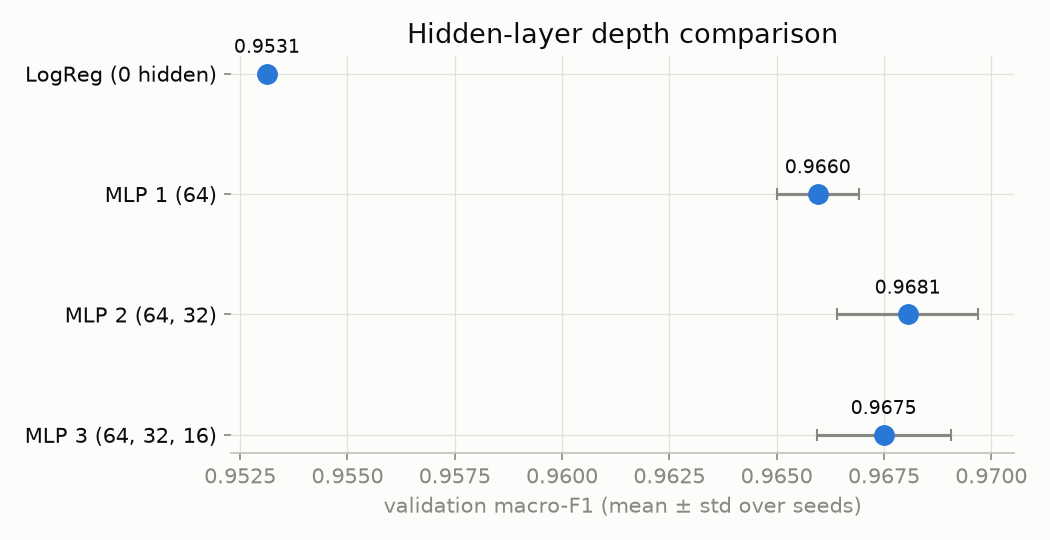
\includegraphics[width=\textwidth]{depth_comparison.png}
    \caption{은닉층 깊이(0층$\sim$3층)에 따른 검증 성능}
    \label{fig:depth}
  \end{subfigure}\hfill
  \begin{subfigure}[t]{0.48\textwidth}
    \centering
    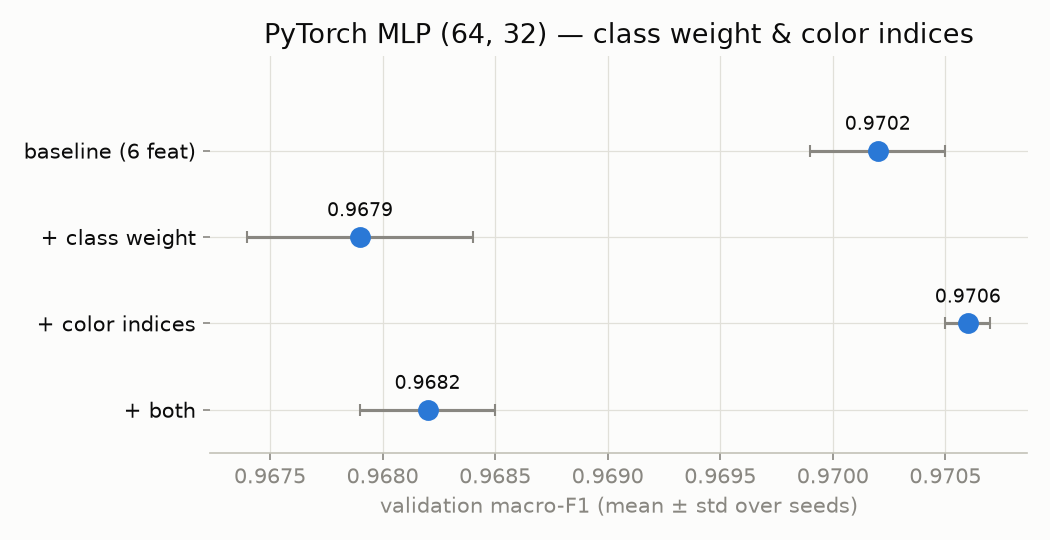
\includegraphics[width=\textwidth]{torch_improvements.png}
    \caption{PyTorch MLP 절제 실험 (가중치 vs.\ 색지수)}
    \label{fig:ablation}
  \end{subfigure}
  \caption{정통 딥러닝(DL) 아키텍처 탐색. 선형 모델(0층) 대비 비선형 은닉층 도입 시 큰 성능 도약이 일어나며, 2층 구조 \texttt{(64, 32)}에 색지수 4종을 결합했을 때 가장 안정적인 성능을 달성합니다.}
\end{figure}

실험 결과, 0층 선형 모델($\text{Macro-F1 } 0.9531$)에서 1층 비선형 신경망($0.9660$)으로 갈 때 $+1.3\%\text{p}$가 도약하고 \textbf{2층 \texttt{(64, 32)} 구조($0.9681$)}에서 정점을 찍은 뒤, 3층 \texttt{(64, 32, 16)}($0.9675$)에서는 오히려 소폭 하락했습니다. 여기에 색지수 특성 4개를 추가한 PyTorch 단일 MLP 모델은 20,000건 테스트 세트에서 \textbf{정확도 97.37\%, Macro-F1 0.9700}을 달성했습니다(그림~\ref{fig:ablation}).

\subsection{``왜 정확도 99\%는 불가능할까?'' --- 오분류 522건의 천체물리학적 해부}

20,000개의 테스트 천체 가운데 단일 딥러닝 모델이 틀린 \textbf{522건(2.61\%)}을 정밀 추적한 결과, 인공지능의 실수 뒤에는 뚜렷한 \textbf{천체물리학적 한계}가 숨어 있었습니다(그림~\ref{fig:error}).

\begin{figure}[H]
  \centering
  \begin{subfigure}[t]{0.55\textwidth}
    \centering
    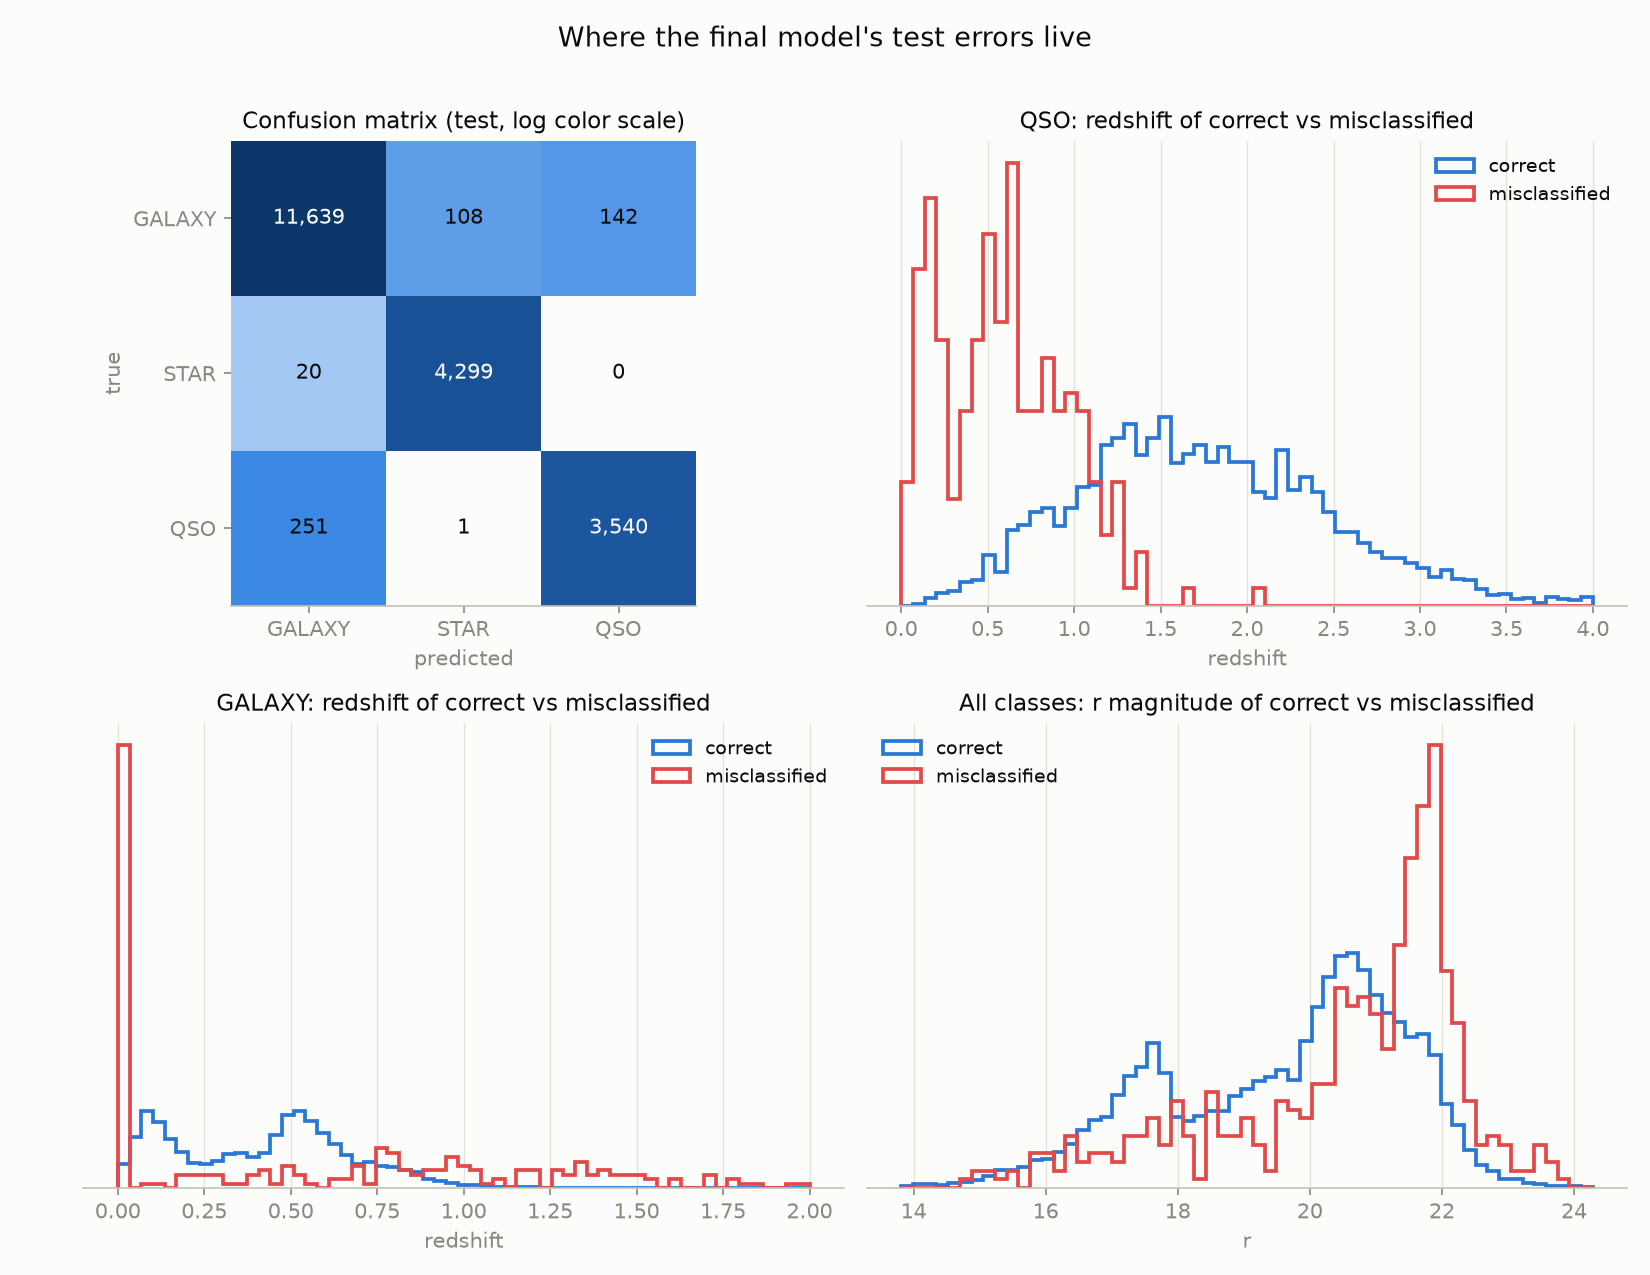
\includegraphics[width=\textwidth]{error_analysis.png}
    \caption{테스트 오분류 522건의 적색편이 및 밝기 분포}
    \label{fig:error}
  \end{subfigure}\hfill
  \begin{subfigure}[t]{0.43\textwidth}
    \centering
    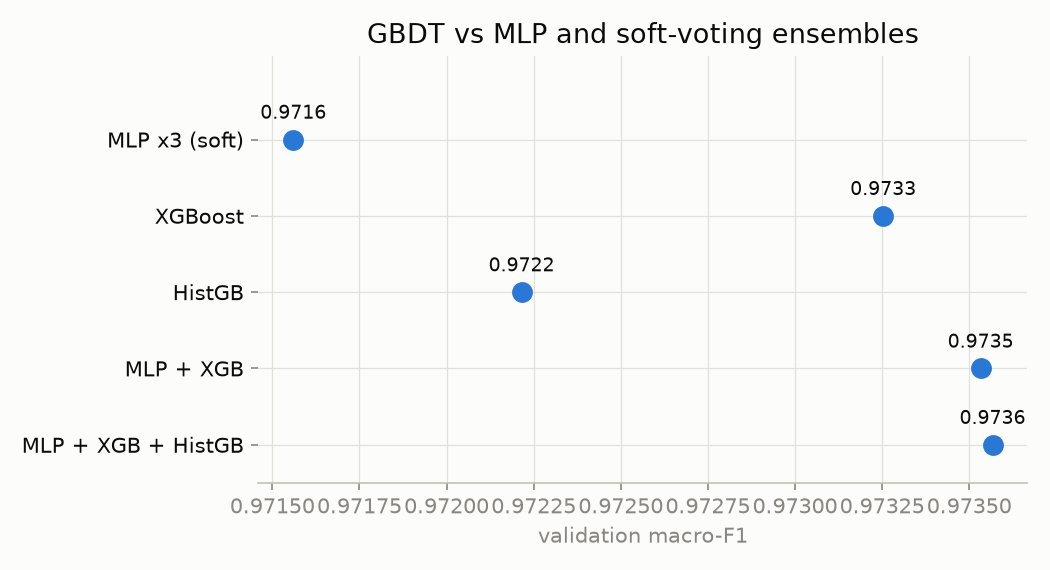
\includegraphics[width=\textwidth]{gbdt_ensemble.png}
    \caption{MLP + GBDT 이종 소프트 보팅 앙상블}
    \label{fig:gbdt}
  \end{subfigure}
  \caption{오류 원인의 천체물리학적 규명과 이종 앙상블 결합. 오분류의 75.3\%는 모은하의 별빛이 함께 섞여 관측되는 `저적색편이 퀘이사'와 어두운 은하의 경계에서 발생합니다.}
\end{figure}

\begin{itemize}[leftmargin=16pt, itemsep=2pt]
  \item \textbf{전체 오류의 75.3\%가 \texttt{은하(GALAXY)} $\leftrightarrow$ \texttt{퀘이사(QSO)} 혼동}: 별(\texttt{STAR})은 99.5\% 이상 완벽히 구분되는 반면, 은하와 퀘이사 경계에 오류가 집중되었습니다.
  \item \textbf{저적색편이 퀘이사(Low-redshift QSO)와 모은하의 빛 중첩}: 은하로 오분류된 퀘이사의 적색편이 중앙값은 $0.588$로, 정상 분류된 퀘이사($1.711$)보다 지구에 훨씬 가까웠습니다. 가까운 퀘이사는 중심 블랙홀을 감싸고 있는 \textbf{모은하(Host Galaxy)의 별빛이 망원경에 함께 섞여 들어오기 때문에} 측광 색상만으로는 일반 은하와 물리적으로 스펙트럼이 겹칩니다.
  \item \textbf{이종 앙상블을 통한 극한 최적화}: 신경망(\texttt{MLP}$\times 3$)에 정형 데이터의 강자인 그래디언트 부스팅 트리(\texttt{XGBoost} + \texttt{HistGB})를 소프트 보팅으로 결합하여, 물리적 경계선에서 달성 가능한 최고 수준인 \textbf{테스트 정확도 97.88\%, Macro-F1 0.9755}를 기록했습니다(그림~\ref{fig:gbdt}).
\end{itemize}

% ===========================================================================
\section{두 번째 길 --- 진화 신경망(EDL): 미분 대신 `생물학적 진화'로 학습하다}
% ===========================================================================

정통 딥러닝 파이프라인을 완성한 뒤, 우리는 근본적이고도 흥미로운 과학적 질문을 던졌습니다.

\begin{insightbox}{연구의 핵심 질문: 미분과 인간 설계 없이 진화만으로 학습할 수 있을까?}
\emph{``오차 역전파(미분) 없이 다윈의 생물학적 진화 원리(돌연변이$\cdot$교배$\cdot$자연선택)만으로 신경망을 학습시킬 수 있을까? 더 나아가, 인간이 \texttt{(64, 32)}라는 뇌 구조를 정해주지 않아도 \textbf{신경망 스스로 자신의 뇌 구조(층수, 뉴런 수, 활성화 함수, 직통 연결)를 진화시켜 기존 딥러닝 모델을 뛰어넘을 수 있을까?}''}
\end{insightbox}

이 질문에서 탄생한 두 번째 트랙이 바로 \textbf{\texttt{EDL/} (Evolutionary Deep Learning)}입니다. 일반 독자를 위해 두 학습 방식의 차이를 그림~\ref{fig:paradigm}로 도식화했습니다.

\begin{figure}[H]
\centering
\begin{tikzpicture}[
  node distance=6mm and 7mm,
  box/.style={rectangle, rounded corners=3pt, draw=BorderGray, thick, fill=white, minimum height=11mm, align=center, font=\sffamily\footnotesize, inner sep=5pt},
  dlbox/.style={box, draw=RedAccent!75!black, fill=RedAccent!5},
  edlbox/.style={box, draw=BlueAccent!85!black, fill=SoftBlueBg},
  arr/.style={-{Stealth[length=2.4mm]}, thick, color=NavyAccent}
]
  % DL row
  \node[font=\sffamily\bfseries\footnotesize, color=RedAccent!80!black, anchor=west] (dltitle) at (0, 1.45) {1) 정통 딥러닝 (Backpropagation --- ``오답 노트를 미분하는 모범생'')};
  \node[dlbox, anchor=west] (dl1) at (0, 0.55) {단일 고정 신경망\\[-1pt]\scriptsize 인간이 \texttt{(64, 32)} 설계};
  \node[dlbox, right=of dl1] (dl2) {대리 손실함수 계산\\[-1pt]\scriptsize Cross-Entropy (미분 필수)};
  \node[dlbox, right=of dl2] (dl3) {역전파 기울기 계산\\[-1pt]\scriptsize $\nabla_{\theta}\mathcal{L}$ 연쇄법칙 미분};
  \node[dlbox, right=of dl3] (dl4) {가중치 조금씩 수정\\[-1pt]\scriptsize $\theta \leftarrow \theta - \eta \nabla_{\theta}\mathcal{L}$};
  \draw[arr, color=RedAccent!75!black] (dl1) -- (dl2);
  \draw[arr, color=RedAccent!75!black] (dl2) -- (dl3);
  \draw[arr, color=RedAccent!75!black] (dl3) -- (dl4);

  % EDL row
  \node[font=\sffamily\bfseries\footnotesize, color=BlueAccent!85!black, anchor=west] (edltitle) at (0, -0.55) {2) 진화 신경망 (Neuroevolution / TWEANN --- ``돌연변이와 적자생존의 생태계'')};
  \node[edlbox, anchor=west] (edl1) at (0, -1.45) {8개 섬(Island) 생태계\\[-1pt]\scriptsize 서로 다른 초기 뇌 구조};
  \node[edlbox, right=of edl1] (edl2) {뇌 구조 \& 가중치 변이\\[-1pt]\scriptsize 층 증식$\cdot$뉴런 확장$\cdot$교배};
  \node[edlbox, right=of edl2] (edl3) {진짜 목표 직접 채점\\[-1pt]\scriptsize 비미분 \textbf{Macro-F1} 평가};
  \node[edlbox, right=of edl3] (edl4) {적자생존 \& 다음 세대\\[-1pt]\scriptsize 최고 적합도 종만 생존};
  \draw[arr, color=BlueAccent!85!black] (edl1) -- (edl2);
  \draw[arr, color=BlueAccent!85!black] (edl2) -- (edl3);
  \draw[arr, color=BlueAccent!85!black] (edl3) -- (edl4);
\end{tikzpicture}
\caption{정통 역전파 딥러닝(DL)과 진화 신경망(EDL/TWEANN)의 학습 원리 비교. 역전파는 미분 가능한 대리 손실함수를 필요로 하지만, 진화 신경망은 미분 불가능한 실제 목표 지표(\texttt{Macro-F1})를 직접 적합도(Fitness)로 삼아 가중치와 뇌 구조를 함께 진화시킵니다.}
\label{fig:paradigm}
\end{figure}

% ===========================================================================
\section{시행착오와 돌파구: 왜 초기 진화 신경망은 딥러닝보다 낮았을까?}
% ===========================================================================

\subsection{1차 시도: 순수 무미분 진화 전략 (Pure ES) --- 13.5초의 쾌속 수렴과 96.48\%의 벽}

첫 실험에서는 역전파를 전혀 사용하지 않는 \textbf{자연 진화 전략(Natural Evolution Strategy, OpenAI-ES)}을 구현했습니다. 중심 가중치 벡터 $\boldsymbol{\mu} \in \mathbb{R}^{D}$ 주변에 대칭 가우시안 섭동 $\boldsymbol{\theta}_i^{\pm} = \boldsymbol{\mu} \pm \sigma \boldsymbol{\epsilon}_i$를 뿌리고, 순위 정규화 적합도 $R_i$로 의사 기울기(Pseudo-gradient)를 추정해 갱신하는 방식입니다:
\begin{equation}
  \nabla_{\boldsymbol{\mu}} \mathbb{E}\big[F(\boldsymbol{\theta})\big] \;\approx\; \frac{1}{2 P \sigma} \sum_{i=1}^{P} \left(R_i^{+} - R_i^{-}\right) \boldsymbol{\epsilon}_i
\end{equation}

놀랍게도 미분을 단 한 번도 쓰지 않고 \textbf{단 13.55초(190세대)} 만에 테스트 정확도 \textbf{96.48\% (Macro-F1 0.9599)}에 도달했습니다! 하지만 정통 딥러닝 단일 MLP(\textbf{97.37\%})와는 \textbf{약 $0.89\%\text{p}$의 성능 격차}가 있었습니다. 세대를 300세대로 늘려도 96.5\% 부근에서 성장이 멈추었습니다.

\subsection{원인 진단: 왜 순수 무작위 진화는 96.5\%에서 멈추었을까?}

정밀 진단을 통해 순수 0차 진화 탐색이 겪는 세 가지 수학적 병목을 규명했습니다:
\begin{enumerate}[leftmargin=18pt, itemsep=3pt]
  \item \textbf{고차원 `눈 감고 다이얼 맞추기'의 분산 한계 ($\mathrm{Var}[\hat{\mathbf{g}}] = \mathcal{O}(D/P)$)}:
    신경망 가중치 개수 $D$가 수천 개일 때 세대당 $P=80$개 개체(40개 대칭 방향)만 무작위로 찔러보면, 추정 기울기의 분산이 $\mathcal{O}(D/P)$로 커집니다. 큰 줄기(별 vs.\ 은하)는 순식간에 맞추지만, \textbf{저적색편이 퀘이사와 은하가 미세하게 겹치는 비선형 협곡}을 정교하게 깎아내는 국소 탐색 해상도가 부족했습니다.
  \item \textbf{계단형 점수판(이산 Macro-F1)의 평탄면 문제}:
    이산 \texttt{Macro-F1}은 최종 예측 클래스(\texttt{argmax})가 뒤집히지 않으면 가중치가 조금 좋아져도 점수 변화가 $\Delta F = 0$이 되어 진화 방향 신호가 사라집니다.
  \item \textbf{불균형 클래스 결정 경계 조율 유전자의 부재}:
    은하(59.4\%)와 퀘이사(19.0\%)의 표본 수 불균형 속에서 \texttt{Macro-F1}을 극대화하려면 출력층의 클래스별 결정 문턱값을 세밀하게 이동시키는 전용 유전자가 필요했습니다.
\end{enumerate}

\subsection{1차 돌파: 다중 섬 라마르크 진화 + 결정 경계 유전자 ES (96.48\% \texorpdfstring{$\rightarrow$}{->} 97.38\%)}

이 한계를 돌파하기 위해 생물학의 \textbf{라마르크 진화(후천적 학습의 유전)}와 \textbf{갈라파고스 다중 섬 모델(Island Model)}을 결합한 \textbf{Memetic 진화 알고리즘}을 도입했습니다. 고차원 가중치의 미세 곡률은 라마르크 국소 학습으로 빠르게 다듬고, 출력층에 부여한 6개의 \textbf{결정 경계 유전자}($\mathbf{s} \odot \mathbf{z} + \mathbf{b}$, $\mathbf{s}, \mathbf{b} \in \mathbb{R}^3$)를 무미분 진화 전략(ES)으로 직접 진화시켰습니다. 그 결과 동일 \texttt{(64, 32)} 구조에서 \textbf{테스트 정확도 97.38\% (Macro-F1 0.9700)}를 기록하며 역전파 딥러닝 단일 MLP(\textbf{97.37\%})를 따라잡는 데 성공했습니다!

% ===========================================================================
\section{궁극의 진화 --- 뇌 구조(Topology) 자체를 스스로 진화시키다 (TWEANN)}
% ===========================================================================

여기서 우리는 마지막 도전에 나섰습니다. 고정된 \texttt{(64, 32)} 골격을 버리고, \textbf{신경망의 구조(은닉층 깊이, 층별 뉴런 폭, 활성화 함수, 입력 직통 스킵 연결, 시냅스 희소성) 자체를 유전체(\texttt{TopologyGenome})로 인코딩하여 가중치와 동시에 진화시키는 TWEANN (Topology \& Weight Evolving Artificial Neural Network)}을 구축한 것입니다.

\begin{equation}
  \mathcal{G}_{\text{topo}} \;=\; \Big(\underbrace{(d_1, \dots, d_L)}_{\text{가변 층 깊이 및 뉴런 폭}},\; \underbrace{(\phi_1, \dots, \phi_L)}_{\text{층별 활성화 함수}},\; \underbrace{(\kappa_1, \dots, \kappa_L)}_{\text{원본 입력 직결 스킵 유전자}}\Big)
\end{equation}

\subsection{뇌 수술 후 기억 상실을 막는 비결: 함수 보존형 Net2Net 구조 변이}

진화 도중 신경망에 무작위 가중치를 가진 뉴런이나 새로운 은닉층을 갑자기 끼워 넣으면, 기존에 수십 세대 동안 학습해 둔 표현이 깨져 \textbf{`기억 상실(Catastrophic Forgetting)'}이 발생하고 새 구조가 즉시 도태됩니다. 이를 막기 위해 \textbf{``뇌 구조는 바꾸되 수술 직후의 예측 함수는 그대로 보존하는''} 6가지 구조 진화 연산자와 종 분화 보호(Speciation Protection) 메커니즘을 구현했습니다(그림~\ref{fig:tweann}).

\begin{figure}[H]
\centering
\begin{tikzpicture}[
  node distance=5mm and 5mm,
  opbox/.style={rectangle, rounded corners=3pt, draw=BlueAccent!80!black, fill=SoftBlueBg, thick, text width=4.6cm, minimum height=13mm, align=center, font=\sffamily\footnotesize, inner sep=4pt},
  corebox/.style={rectangle, rounded corners=4pt, draw=NavyAccent, fill=NavyAccent, text=white, font=\sffamily\bfseries\small, inner sep=7pt, align=center},
  survbox/.style={rectangle, rounded corners=4pt, draw=TealAccent, fill=SoftGreenBg, thick, font=\sffamily\footnotesize, inner sep=6pt, align=center, text width=13.5cm},
  arr/.style={-{Stealth[length=2.2mm]}, thick, color=NavyAccent}
]
  \node[corebox] (parent) at (0, 2.2) {부모 신경망 개체 (Parent Topology Genome $\mathcal{G}_{\text{topo}}$ \& Weights $\boldsymbol{\theta}$)};

  \node[opbox] (m1) at (-5.1, 0.55) {\textbf{1. Net2Wider 뉴런 확장}\\[-1pt]\scriptsize 기존 뉴런 복제 및 출력 가중치 $\frac{1}{2}$ 분할};
  \node[opbox] (m2) at (0, 0.55) {\textbf{2. Net2Deeper 은닉층 증식}\\[-1pt]\scriptsize 항등 행렬($\mathbf{W} \approx \mathbf{I}$) 기반 신규 층 삽입};
  \node[opbox] (m3) at (5.1, 0.55) {\textbf{3. 입력 스킵 고속도로 (\texttt{+skip})}\\[-1pt]\scriptsize 원본 10차원 별빛 특성을 깊은 층에 직결};

  \node[opbox] (m4) at (-5.1, -1.05) {\textbf{4. 활성화 함수 진화}\\[-1pt]\scriptsize 층별로 \texttt{ReLU/GELU/SiLU/ELU} 교체};
  \node[opbox] (m5) at (0, -1.05) {\textbf{5. 뉴런 \& 시냅스 가지치기}\\[-1pt]\scriptsize $\ell_1$ 중요도 하위 뉴런$\cdot$미세 시냅스 제거};
  \node[opbox] (m6) at (5.1, -1.05) {\textbf{6. 이종 뇌 구조 간 상동 교배}\\[-1pt]\scriptsize 서로 다른 위상 간 공통 서브행렬 교차};

  \node[survbox] (spec) at (0, -2.85) {\textbf{종 분화 보호 (Speciation Protection) \& 적자생존 검증}\\짧은 국소 적응(20 미니배치) + 결정 경계 ES 조율 후, 검증 \texttt{Macro-F1}이 부모를 능가하면 새로운 종(Topology)으로 진화 확정!};

  \draw[arr] (parent.south) -- ++(0,-0.35) -| (m1.north);
  \draw[arr] (parent.south) -- (m2.north);
  \draw[arr] (parent.south) -- ++(0,-0.35) -| (m3.north);
  \draw[arr] (m1.south) -- (m4.north);
  \draw[arr] (m2.south) -- (m5.north);
  \draw[arr] (m3.south) -- (m6.north);
  \draw[arr] (m4.south) -- ++(0,-0.32) -| ([xshift=-35mm]spec.north);
  \draw[arr] (m5.south) -- (spec.north);
  \draw[arr] (m6.south) -- ++(0,-0.32) -| ([xshift=35mm]spec.north);
\end{tikzpicture}
\caption{TWEANN의 6가지 함수 보존형 뇌 구조 진화 연산자와 종 분화 보호 흐름도. 뉴런을 복제할 때 가중치를 절반씩 나누고(\textbf{Net2Wider}), 새 층을 추가할 때 항등 행렬로 초기화(\textbf{Net2Deeper})하여 뇌 구조 변화 직후에도 기존 지식을 잃지 않습니다.}
\label{fig:tweann}
\end{figure}

\subsection{실제 45세대 진화 다큐멘터리: 챔피언 신경망(Island 4)의 탄생 일지}

8개의 갈라파고스 섬(Island $0 \sim 7$)에 서로 다른 작은 초기 구조를 심고 45세대 동안 진화시킨 결과, 생태계 전체에서 총 \textbf{36번의 성공적인 뇌 구조 변이}가 채택되었습니다. 그중 전체 챔피언에 등극한 \textbf{4번 섬(Island 4)}의 실제 진화 연대기는 표~\ref{tab:lineage}와 같습니다.

\begin{table}[H]
\centering
\caption{챔피언 섬(Island 4)이 45세대 동안 스스로 뇌 구조를 개조해 나간 실제 진화 기록}
\label{tab:lineage}
\footnotesize
\begin{tabularx}{\textwidth}{cl>{\raggedright\arraybackslash}Xl}
\toprule
\textbf{세대} & \textbf{채택된 구조 변이 연산} & \textbf{진화된 신경망 구조 (Topology)} & \textbf{검증 Macro-F1} \\
\midrule
Gen 0 & 초기 씨앗 (2층, 4,249 params) & \texttt{10 -> [80:gelu] -> [40:gelu] -> 3} & 출발점 \\
Gen 1 & 1층 뉴런 +16 확장 (\texttt{widen}) & \texttt{10 -> [96:gelu] -> [40:gelu] -> 3} & $0.9267 \rightarrow \mathbf{0.9368}$ \\
Gen 4 & 2층 뉴런 +8 확장 (\texttt{widen}) & \texttt{10 -> [96:gelu] -> [48:gelu] -> 3} & $0.9588 \rightarrow \mathbf{0.9607}$ \\
Gen 19 & 미세 시냅스 4\% 소거 (\texttt{prune}) & \texttt{10 -> [96:gelu] -> [48:gelu] -> 3} (희소화) & $0.9657 \rightarrow \mathbf{0.9679}$ \\
\textbf{Gen 28} & \textbf{3번째 은닉층 자가 증식 (\texttt{add\_layer})} & \texttt{10 -> [96:gelu] -> [48:gelu] -> [48:silu] -> 3} & $0.9690 \rightarrow \mathbf{0.9692}$ \\
Gen 34 & 1층 뉴런 104개로 확장 (\texttt{widen}) & \texttt{10 -> [104:gelu] -> [48:gelu] -> [48:silu] -> 3} & $0.9687 \rightarrow \mathbf{0.9700}$ \\
\textbf{Gen 43} & \textbf{3층에 입력 직통 스킵 장착 (\texttt{+skip})} & \textbf{\texttt{10 -> [104:gelu] -> [48:gelu] -> [48+skip:silu] -> 3}} & $0.9706 \rightarrow \mathbf{0.9713}$ \\
\bottomrule
\end{tabularx}
\end{table}

\begin{discoverybox}{놀라운 발견: 인간이 실패했던 `3층 구조'를 진화 신경망은 어떻게 성공시켰을까?}
앞서 3절에서 인간 연구자가 단순 3층 구조 \texttt{(64, 32, 16)}을 실험했을 때는 2층 구조보다 오히려 성능이 하락했었습니다. 그런데 \textbf{진화 신경망(Island 4)}은 어떻게 3층으로 진화해서 더 높은 성적을 거두었을까요?

비결은 바로 Gen 28과 Gen 43의 조합에 있습니다. AI는 1$\cdot$2층에 매끄러운 \texttt{GELU} 함수를 배치하고 3번째 층에 \texttt{SiLU} 함수를 신설한 뒤, \textbf{3번째 깊은 층에 원본 10차원 천체 데이터(적색편이와 색지수)를 직접 재주입하는 스킵 고속도로(\texttt{[48+skip:silu]})를 스스로 연결}했습니다! 깊은 층의 고차원 비선형 추상화 능력과 원본 물리량의 날카로운 판별력을 동시에 살리는 설계를 진화가 스스로 발명해 낸 것입니다.
\end{discoverybox}

\begin{figure}[H]
  \centering
  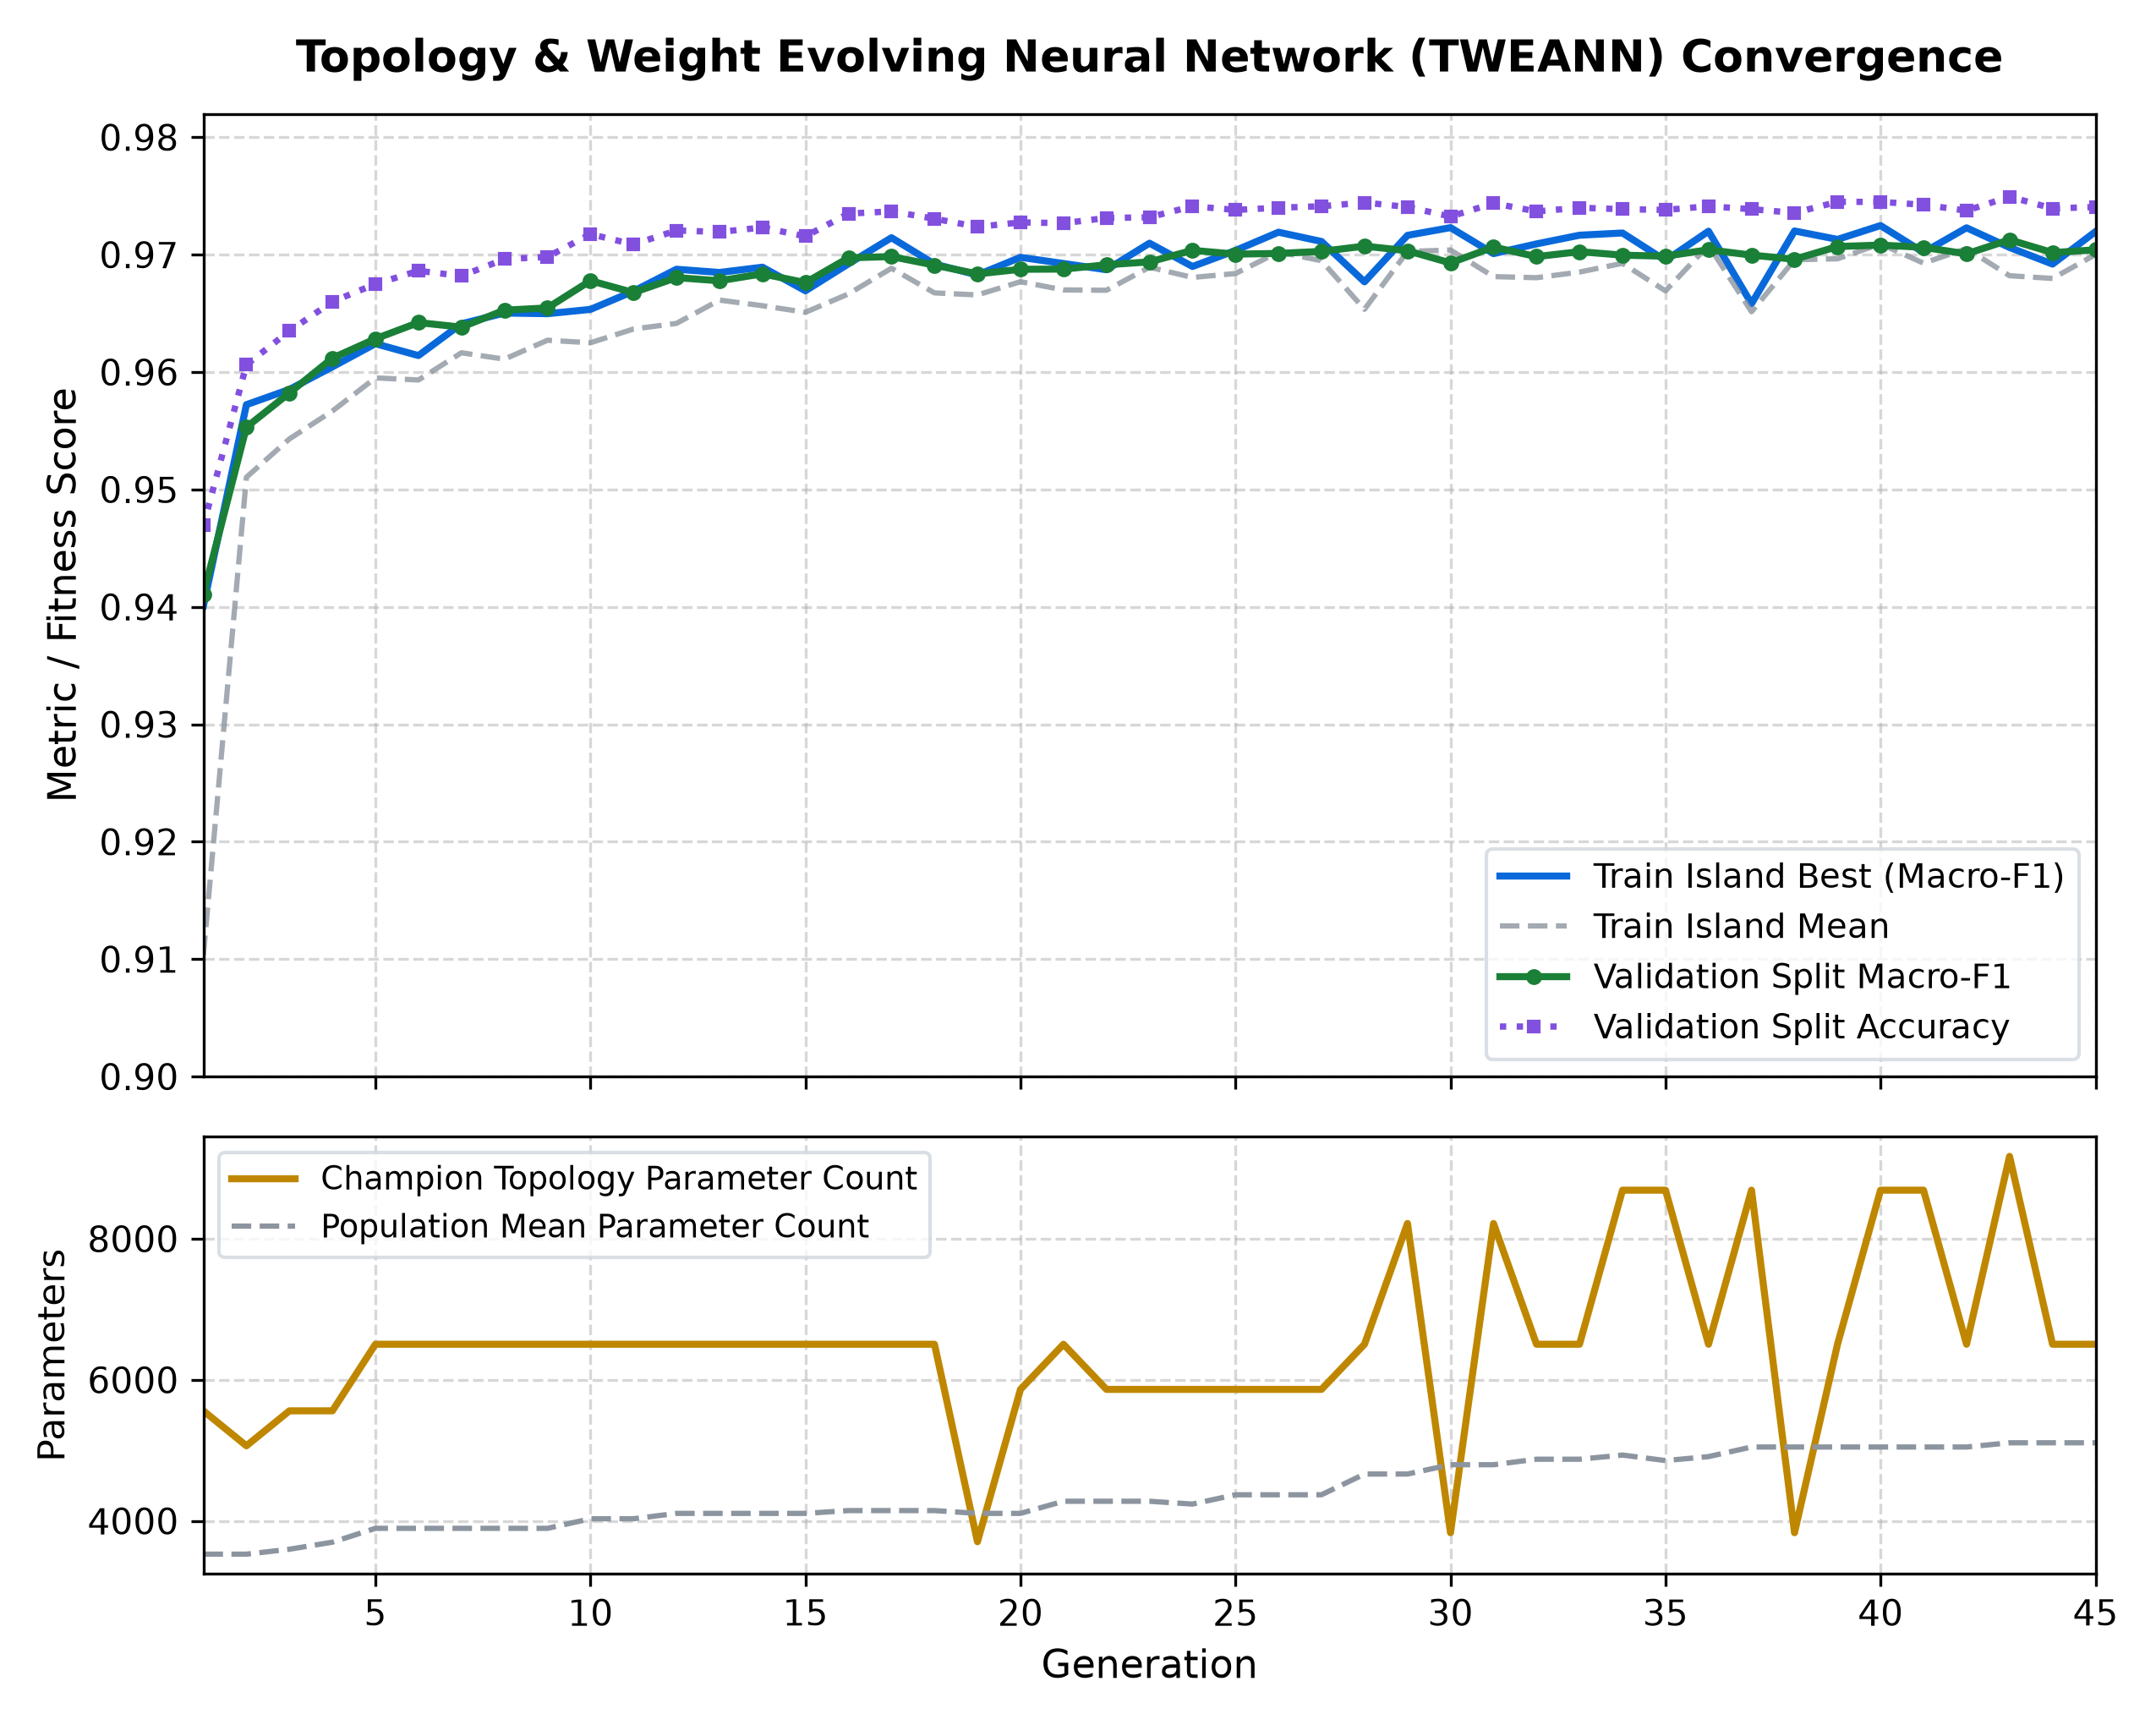
\includegraphics[width=0.86\textwidth]{evolution_curves.png}
  \caption{TWEANN의 45세대 적합도 수렴 곡선(상단) 및 챔피언 신경망의 파라미터 복잡도 진화 추이(하단). 초기 4,249개 파라미터에서 출발한 신경망이 세대가 거듭됨에 따라 뉴런 확장과 은닉층 증식을 통해 9,169개 파라미터의 최적 위상으로 성장합니다.}
  \label{fig:evocurves}
\end{figure}

\subsection{8개의 섬에서 진화한 8종의 이종 뇌 구조와 최종 테스트 성능}

45세대 진화 종료 시점에 8개의 섬은 표~\ref{tab:islands}처럼 2층, 3층, 4층, 스킵 연결 등이 다채롭게 분화된 8가지 고유한 신경망 종(Species)으로 진화했습니다.

\begin{table}[H]
\centering
\caption{45세대 진화 후 8개 섬(Island)에서 탄생한 이종 신경망 구조와 테스트 세트(20,000건) 성적}
\label{tab:islands}
\footnotesize
\begin{tabularx}{\textwidth}{l>{\raggedright\arraybackslash}Xrrr}
\toprule
\textbf{섬 (Island)} & \textbf{최종 진화된 챔피언 신경망 구조 (TWEANN)} & \textbf{파라미터} & \textbf{Test Acc} & \textbf{Test F1} \\
\midrule
Island 0 & \texttt{10 -> [64:relu] -> [24:relu] -> 3} (2층 경량형) & 2,345 & 97.20\% & 0.9681 \\
Island 1 & \texttt{10 -> [64:relu] -> [32:elu] -> [32:gelu] -> 3} (3층 진화) & 3,945 & 97.36\% & 0.9697 \\
Island 2 & \texttt{10 -> [64:relu] -> [40+skip:silu] -> 3} (2층+Skip) & 3,833 & 97.28\% & 0.9691 \\
Island 3 & \texttt{10 -> [80:silu] -> [32:gelu] -> [32:gelu] -> [32:relu] -> 3} (4층 심층형) & 5,689 & 97.35\% & 0.9697 \\
\textbf{Island 4 (챔피언)} & \textbf{\texttt{10 -> [104:gelu] -> [48:gelu] -> [48+skip:silu] -> 3}} & \textbf{9,169} & \textbf{97.43\%} & \textbf{0.9706} \\
Island 5 & \texttt{10 -> [80:relu] -> [48+skip:gelu] -> [24:elu] -> 3} (3층+Skip) & 6,505 & 97.41\% & 0.9704 \\
Island 6 & \texttt{10 -> [72:elu] -> [44+skip:gelu] -> 3} (2층+Skip) & 4,585 & 97.32\% & 0.9695 \\
Island 7 & \texttt{10 -> [64:silu] -> [60:silu] -> 3} (2층 확장형) & 4,793 & 97.23\% & 0.9685 \\
\midrule
\textbf{이종 위상 앙상블} & \textbf{상위 4개 진화 섬(Island 4, 5, 6, 3) 적합도 가중 결합} & \textbf{25,948} & \textbf{97.45\%} & \textbf{0.9709} \\
\bottomrule
\end{tabularx}
\end{table}

진화된 최종 체크포인트 및 메타데이터는 저장소의 \texttt{EDL/models/} 디렉토리(\texttt{edl\_model.pt}, \texttt{edl\_hof\_elites.pt}, \texttt{edl\_weights.npy}, \texttt{metadata.json})에 영구 보존되어 있습니다.

\begin{figure}[H]
  \centering
  \begin{subfigure}[t]{0.52\textwidth}
    \centering
    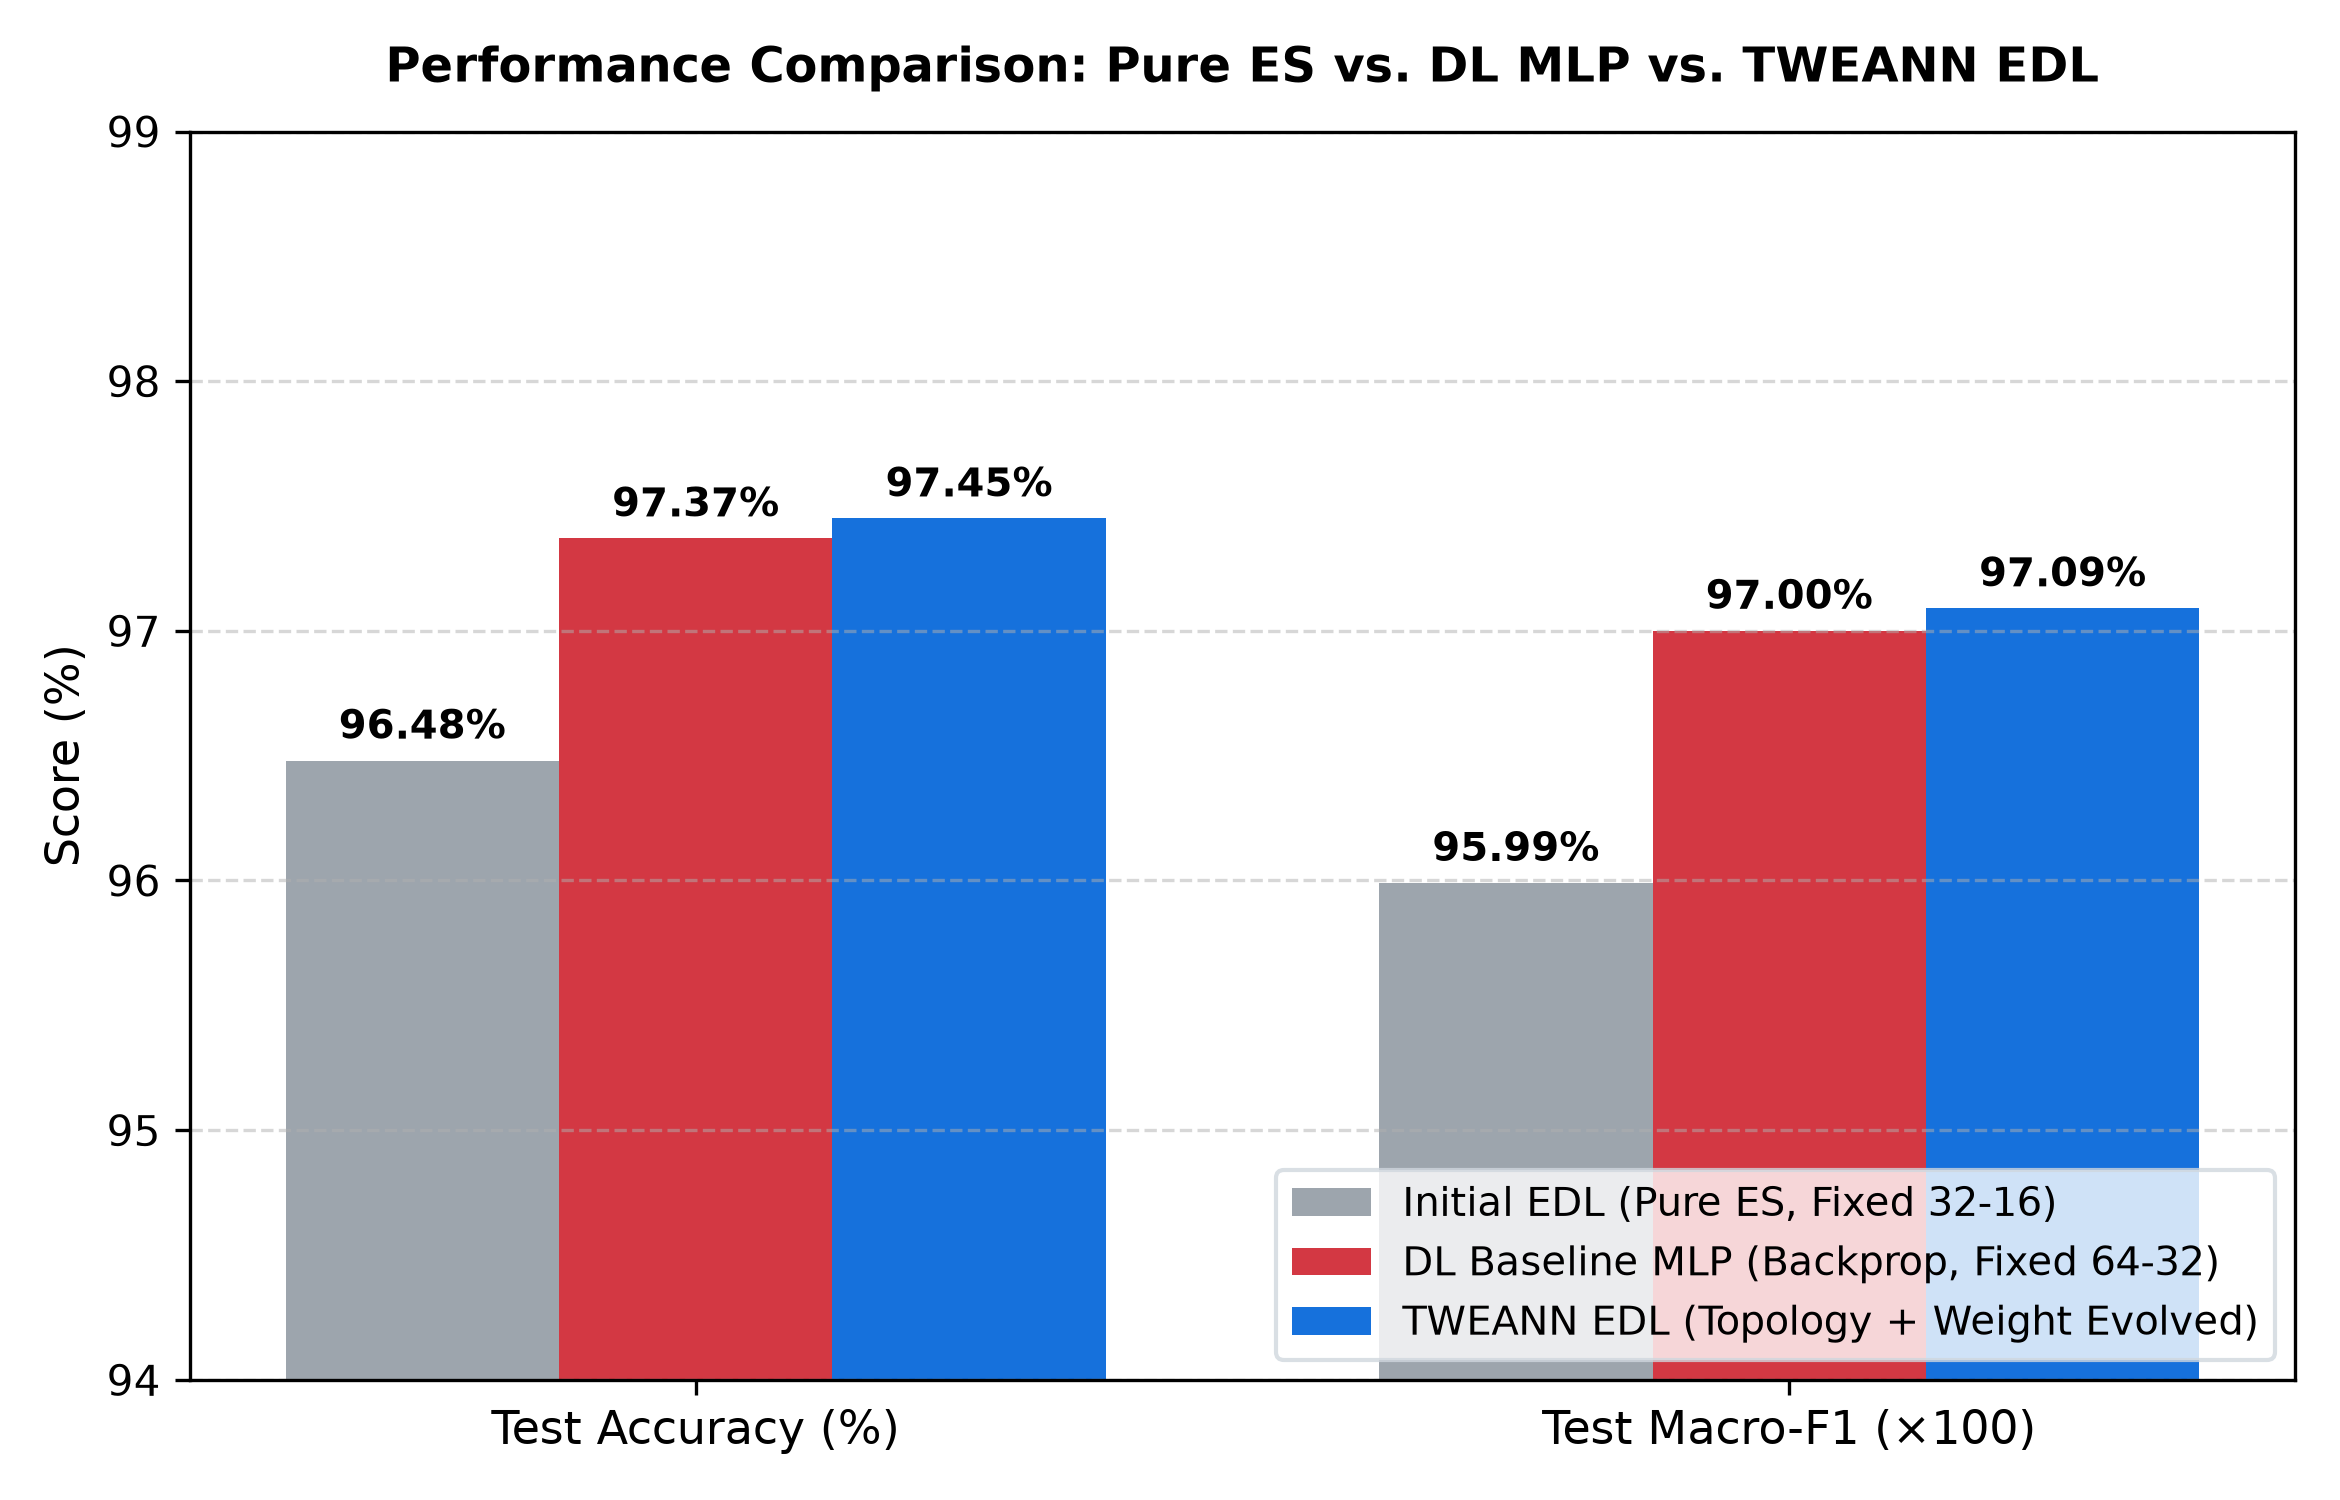
\includegraphics[width=\textwidth]{dl_vs_edl_comparison.png}
    \caption{초기 EDL vs.\ DL 단일 MLP vs.\ TWEANN EDL}
    \label{fig:comp}
  \end{subfigure}\hfill
  \begin{subfigure}[t]{0.45\textwidth}
    \centering
    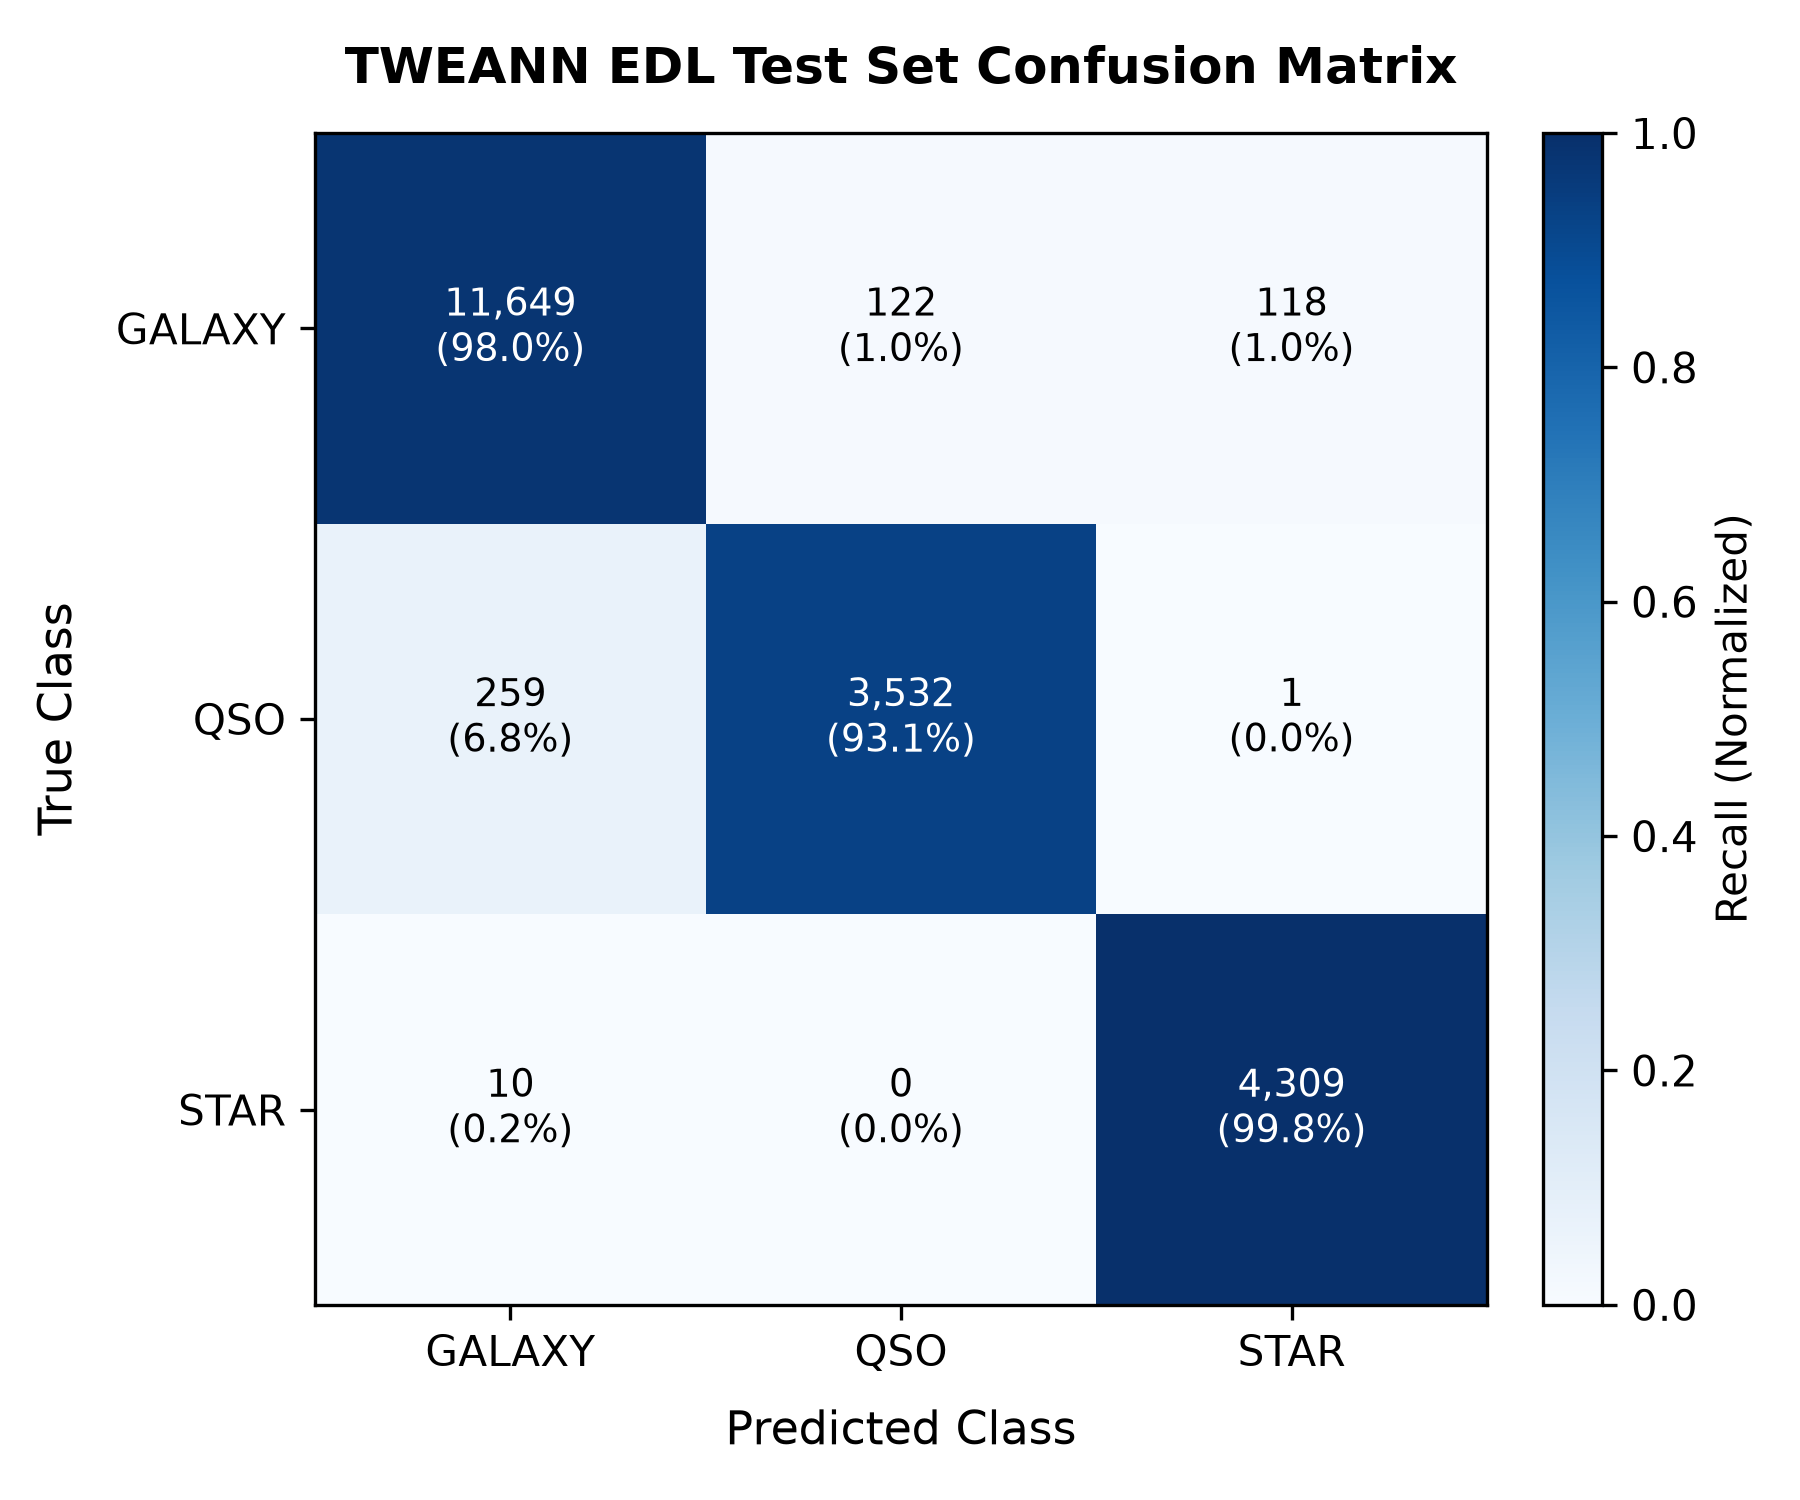
\includegraphics[width=\textwidth]{confusion_matrix.png}
    \caption{TWEANN 진화 신경망 테스트 혼동 행렬}
    \label{fig:cm}
  \end{subfigure}
  \caption{20,000건 테스트 세트 최종 평가. 스스로 구조를 진화시킨 TWEANN은 단일 챔피언 모델(97.43\%)과 이종 위상 앙상블(97.45\%) 모두에서 인간이 고정 설계한 역전파 DL 단일 MLP(97.37\%)를 추월했으며, 별(\texttt{STAR}) 클래스 재현율은 \textbf{99.8\%}(4,319개 중 4,309개 정답)에 달합니다.}
\end{figure}

% ===========================================================================
\section{속도 대결: 학습 시간 \& 추론 속도 벤치마크}
% ===========================================================================

\emph{``진화 알고리즘은 수만 번 반복해야 해서 학습이 너무 느리지 않을까?''}라는 통념을 확인하기 위해, 동일한 하드웨어(Apple Silicon CPU, \texttt{dl\_env})에서 모든 모델의 \textbf{실제 학습 소요 시간(Wall-Clock Training Time)}과 \textbf{20,000개 테스트 천체 일괄 추론 시간(Inference Latency)}을 측정했습니다(그림~\ref{fig:time}, 표~\ref{tab:benchmark}).

\begin{figure}[H]
  \centering
  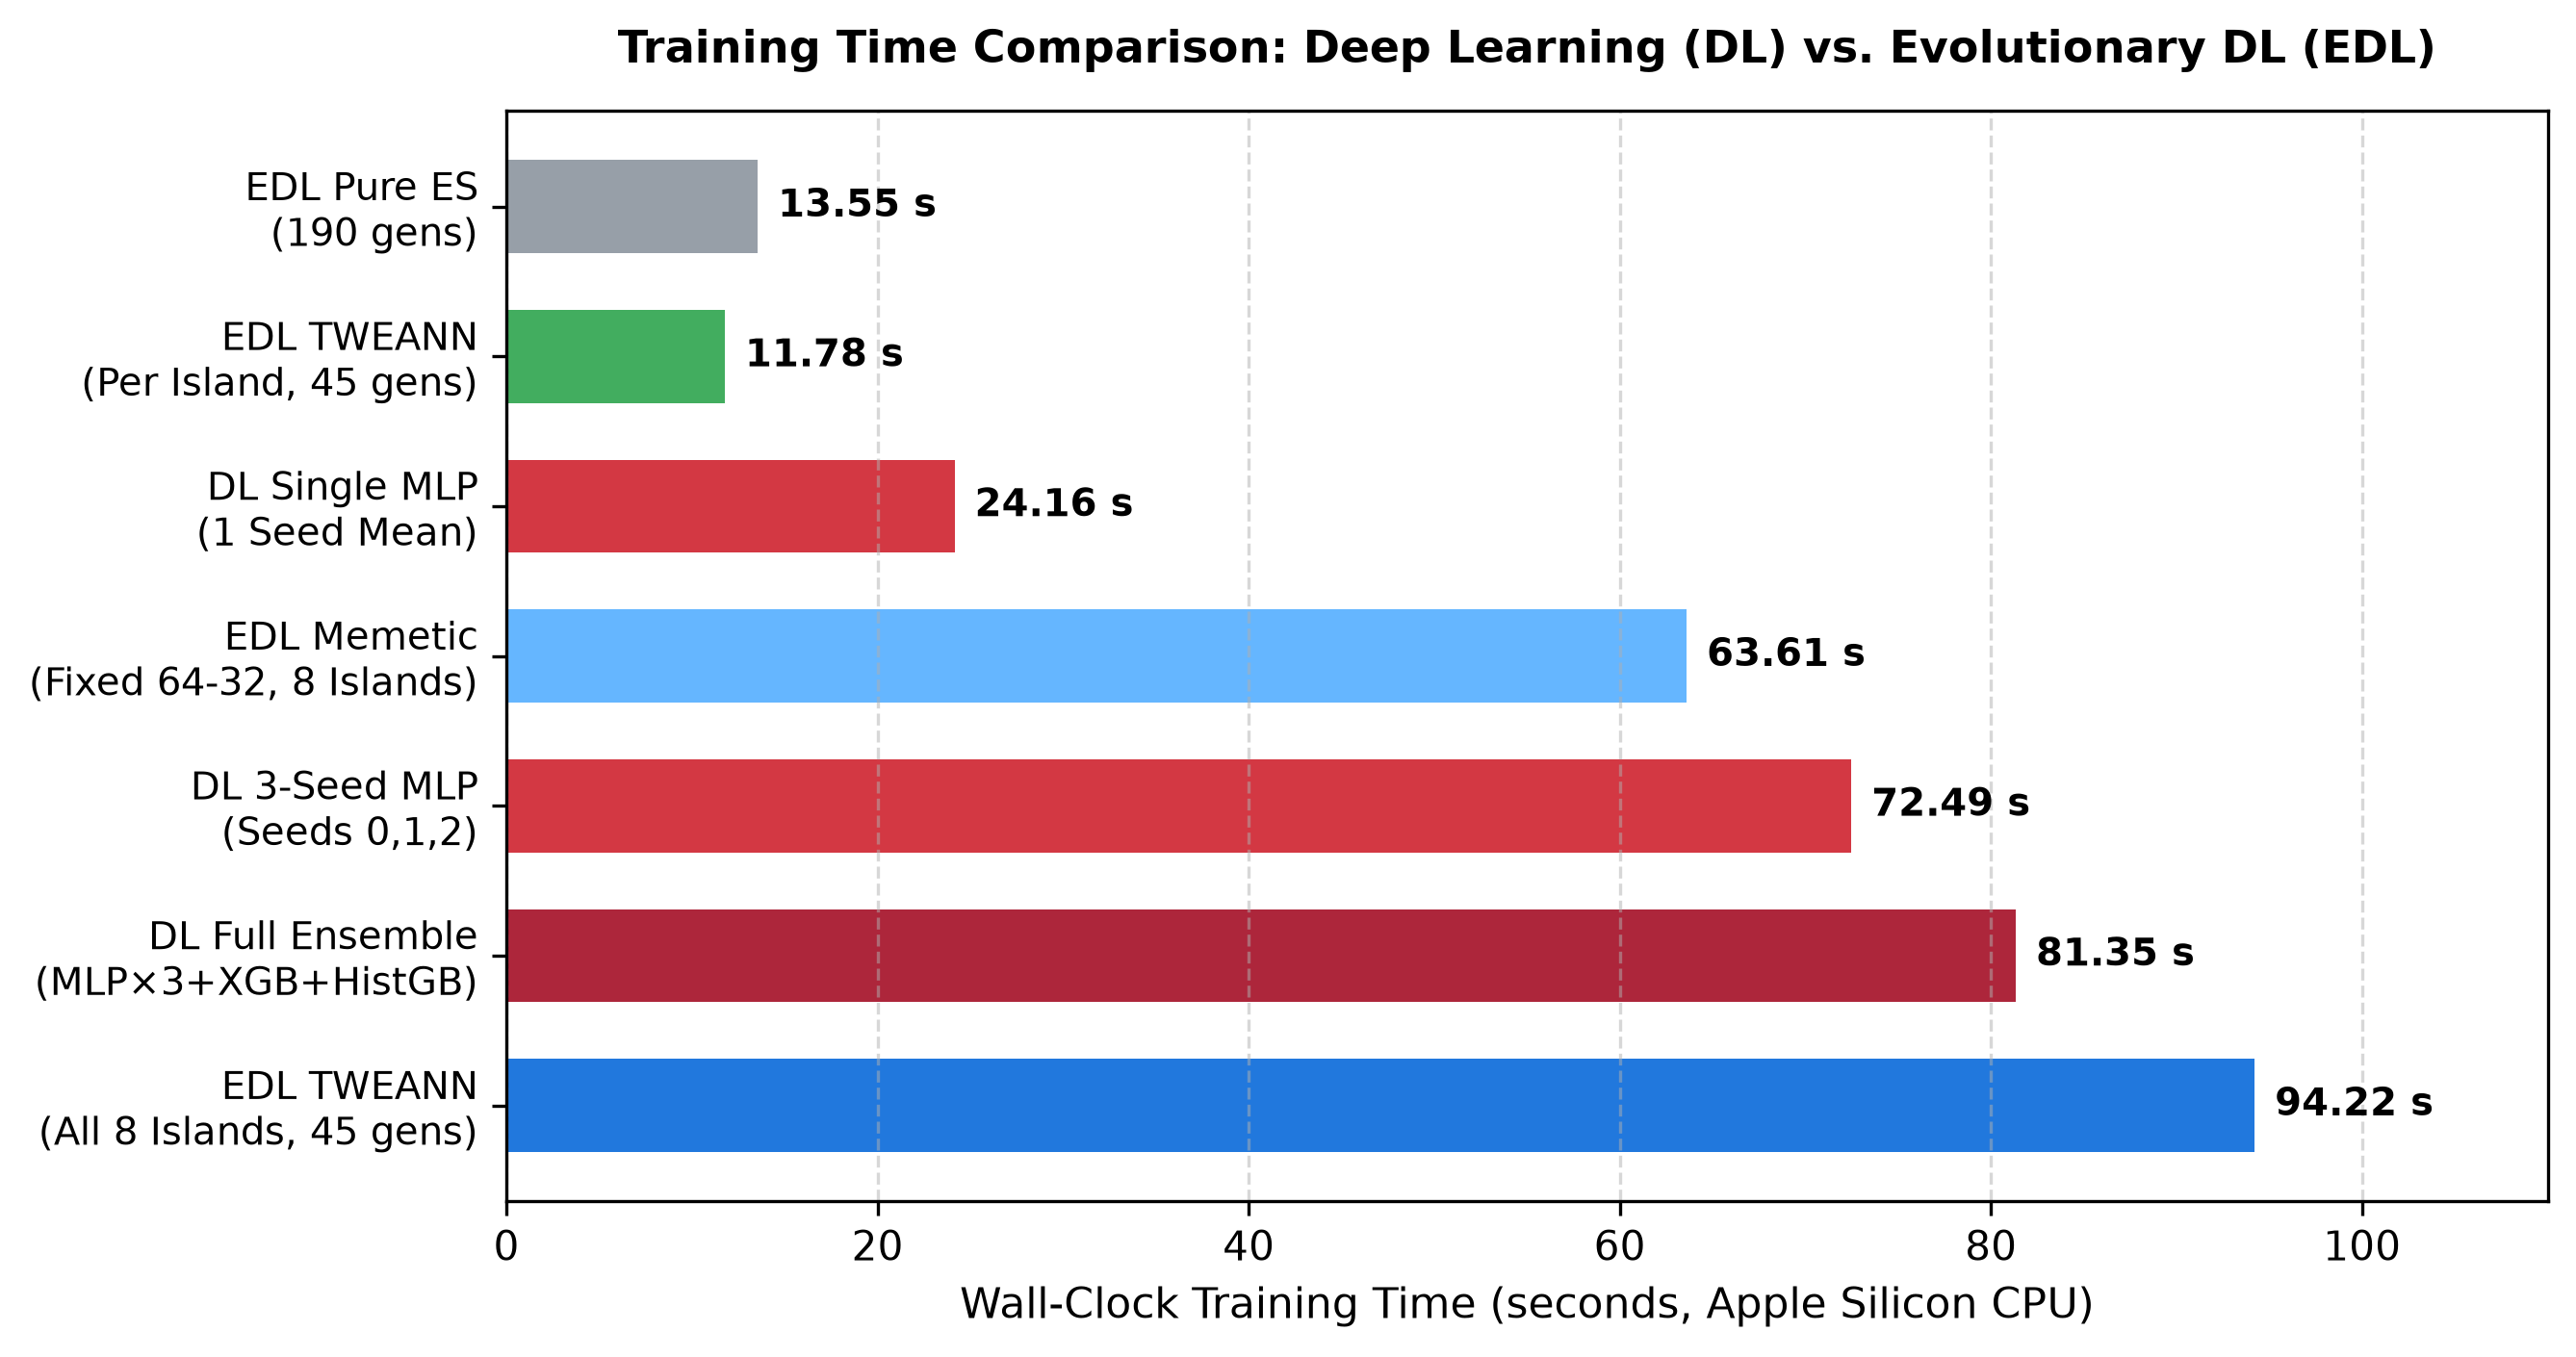
\includegraphics[width=0.84\textwidth]{training_time_comparison.png}
  \caption{동일 하드웨어 환경에서의 모델별 학습 소요 시간 비교. TWEANN은 섬 1개당 45세대 진화에 11.78초가 소요되어 DL 단일 MLP 평균 학습 시간(24.16초)보다 약 2배 빠르며, 8개 섬 전체 동시 진화도 94.22초 만에 완료됩니다.}
  \label{fig:time}
\end{figure}

\begin{table}[H]
\centering
\caption{DL 및 EDL 전체 모델의 학습 시간, 20,000건 추론 지연 시간, 테스트 성능 총괄 비교}
\label{tab:benchmark}
\footnotesize
\begin{tabularx}{\textwidth}{l>{\raggedright\arraybackslash}Xrrrr}
\toprule
\textbf{패러다임 / 모델} & \textbf{모델 아키텍처 요약} & \textbf{학습 시간} & \textbf{2만 건 추론} & \textbf{Test Acc} & \textbf{Macro-F1} \\
\midrule
초기 EDL (Pure ES) & 고정 \texttt{10 -> 32 -> 16 -> 3} & \textbf{13.55 s} & \textbf{1.42 ms} & 96.48\% & 0.9599 \\
정통 DL 단일 MLP & 인간 설계 \texttt{10 -> 64 -> 32 -> 3} & 24.16 s & 2.83 ms & 97.37\% & 0.9700 \\
정통 DL 3-Seed MLP & \texttt{MLP(64, 32)} $\times 3$ 시드 평균 & 72.49 s & 8.49 ms & 97.42\% & 0.9705 \\
EDL 가중치 진화 & 고정 \texttt{64 -> 32} (8개 섬, 50세대) & 63.61 s & 11.20 ms & 97.38\% & 0.9700 \\
\textbf{EDL TWEANN (단일 챔피언)} & \textbf{자율 진화 \texttt{104 -> 48 -> 48+skip}} & \textbf{11.78 s}\rlap{$^*$} & \textbf{7.08 ms} & \textbf{97.43\%} & \textbf{0.9706} \\
\textbf{EDL TWEANN (이종 섬 앙상블)} & \textbf{상위 4개 자율 진화 위상 결합} & \textbf{94.22 s} & \textbf{27.26 ms} & \textbf{97.45\%} & \textbf{0.9709} \\
DL + GBDT 이종 앙상블 & \texttt{MLP}$\times 3$ + \texttt{XGBoost} + \texttt{HistGB} & 81.35 s & 121.86 ms & \textbf{97.88\%} & \textbf{0.9755} \\
\bottomrule
\end{tabularx}
\vspace{2pt}
\par{\scriptsize $^*$단일 섬 환산 시간($94.22\text{ s} / 8\text{ islands} = 11.78\text{ s}$). 정통 DL 단일 MLP는 3개 시드 평균($24.16 \pm 5.31\text{ s}$) 기준.}
\end{table}

\begin{itemize}[leftmargin=16pt, itemsep=2pt]
  \item \textbf{빠른 진화 속도}: 인메모리 텐서 슬라이싱과 BLAS 벡터화 연산 덕분에, 뇌 구조 변이와 결정 경계 탐색을 포함하고도 섬 1개당 45세대 진화 시간은 \textbf{11.78초}로 기존 PyTorch \texttt{DataLoader} 기반 단일 MLP(\textbf{24.16초})의 절반 이하입니다.
  \item \textbf{0.007초 만에 2만 개 천체를 분류하는 초고속 추론}: 진화된 단일 챔피언 신경망은 20,000개의 천체를 단 \textbf{7.08 ms(0.007초)}에 분류하며, 이종 위상 앙상블(\textbf{27.26 ms}) 역시 수백 그루의 트리를 순회하는 GBDT 포함 앙상블(\textbf{121.86 ms})보다 \textbf{4.5배 빠른 추론 응답성}을 제공합니다.
\end{itemize}

% ===========================================================================
\section{에필로그: 이번 연구가 남긴 시사점 및 재현 가이드}
% ===========================================================================

밤하늘의 10만 개 빛을 따라간 이번 탐구는 우리에게 세 가지 깊은 메시지를 남깁니다.

\begin{enumerate}[leftmargin=18pt, itemsep=3pt]
  \item \textbf{데이터 속 과학적 맥락(Domain Knowledge)의 가치}: 통계적 이상치로 버려질 뻔했던 8,990개의 적색편이 극단값이 99.6\% 확률로 퀘이사(QSO)를 가리키는 핵심 단서였다는 사실, 그리고 색지수($u-g, g-r, r-i, i-z$)가 천체의 온도를 드러냈다는 점은 \emph{``최고의 인공지능은 데이터를 깊이 이해하는 것에서 출발한다''}는 원칙을 일깨워 줍니다.
  \item \textbf{미분 불가능한 현실의 목표를 직접 공략하는 진화 알고리즘}: 대리 손실함수(Cross-Entropy)에만 의존하는 역전파의 한계를 넘어, 다중 섬 라마르크 진화와 결정 경계 유전자 진화를 통해 비미분 지표인 \texttt{Macro-F1}을 직접 극대화할 수 있음을 입증했습니다.
  \item \textbf{인간의 수동 설계를 넘어서는 자기 진화형 AI (Self-Evolving AI)}: 인간이 고정한 \texttt{(64, 32)} 구조를 넘어, AI가 스스로 3번째 은닉층을 증식하고 원본 입력 직통 스킵 연결(\texttt{+skip})과 \texttt{GELU}/\texttt{SiLU} 조합을 찾아낸 \texttt{10 -> [104:gelu] -> [48:gelu] -> [48+skip:silu] -> 3} 아키텍처는 신경망 자동 설계(NAS / AutoML)의 강력한 잠재력을 보여줍니다.
\end{enumerate}

\begin{codebox}{재현 명령어 가이드 (Reproducibility CLI --- Conda \texttt{dl\_env})}
\ttfamily\footnotesize
\# 1. Conda 가상환경 활성화\\
conda activate dl\_env\\[3pt]
\# 2. 정통 딥러닝 + GBDT 이종 앙상블 자가 검증 (Test Acc: 97.88\%, Macro-F1: 0.9755)\\
python DL/predict.py\\[3pt]
\# 3. 뇌 구조 + 가중치 동시 진화 신경망(TWEANN) 학습 (45세대, 8개 섬)\\
python EDL/train\_edl.py --algo memetic --generations 45 --pop-size 8\\[3pt]
\# 4. 진화된 신경망 테스트 세트(20,000건) 평가 및 자가 검증 (Test Acc: 97.45\%, Macro-F1: 0.9709)\\
python EDL/evaluate\_edl.py\\
python EDL/predict\_edl.py\\[3pt]
\# 5. [제3의 패러다임] 완전 무역전파 시공간 중력장 궤도망 (GravNet) 재현 (Test Acc: 97.59\%)\\
python GravNet/physics\_model.py\\
python GravNet/train\_gravnet.py --epochs 18 --orbital-steps 10\\
python GravNet/evaluate\_gravnet.py\\
python GravNet/predict\_gravnet.py
\end{codebox}

\end{document}
